\documentclass[11pt,a4paper]{article}

%% Language and font encodings
\usepackage[utf8]{inputenc}
\usepackage[margin=1in]{geometry}
\usepackage{authblk}
\usepackage[style=apa]{biblatex}
\usepackage[american]{babel}
\usepackage[finalizecache,cachedir=.]{minted}
\usepackage{csquotes}
\DeclareLanguageMapping{american}{american-apa}
\bibliography{references.bib}

\usepackage{amsmath,amsfonts,amssymb,bm,bbm,amsthm}
\usepackage[colorinlistoftodos,textsize=small]{todonotes}
\usepackage{graphicx}
%\usepackage{breqn}
\usepackage{todonotes}
\usepackage{xcolor} % color math symbols, delete later
\usepackage{verbatim}
\newcommand\todoin[2][]{\todo[inline, caption={2do}, #1]{
	\begin{minipage}{\textwidth-4pt}#2\end{minipage}}
}
\usepackage{nicefrac}

\theoremstyle{definition} % no italiced theorem style
\newtheorem{prop}{Proposition}
\newtheorem{corr}{Corollary}[prop]
\newtheorem{lemma}[prop]{Lemma}

\newtheoremstyle{case}{}{}{}{}{}{:}{ }{}
\theoremstyle{case}
\newtheorem{case}{Case}

\usepackage[colorinlistoftodos,textsize=small]{todonotes}
\usepackage[colorlinks=true, allcolors=blue, bookmarks=false]{hyperref}


\newcommand{\iu}{{i\mkern1mu}}
\newcommand{\Lik}{\mathbb{L}}
\newcommand{\bx}{\bm{x}}
\newcommand{\by}{\bm{y}}
\newcommand{\bz}{\bm{z}}
\newcommand{\Reals}{\mathbb{R}}
\newcommand{\dx}[1]{\enspace \mathrm{d}{#1}}
\newcommand{\prior}[1]{\pi\left({#1}\right)}
\newcommand{\FGamma}[1]{\Gamma\left({#1}\right)}
\newcommand{\FBeta}[2]{\text{B}\left({#1},\ {#2}\right)}
\newcommand{\FHyperG}[1]{\, _2F_1\left({#1}\right)}
\newcommand{\FHyperGn}{\, _2F_1}
\newcommand{\mean}[1]{\overline{{#1}}}
\newcommand{\Lim}[1]{\raisebox{0.5ex}{\scalebox{0.8}{$\displaystyle \lim_{#1}\;$}}}
\newcommand{\BF}{\text{BF}}
\newcommand{\FHypGeo}[4]{\,_2F_1\left({#1};{#2};{#3};{#4}\right)}
\newcommand{\BetaBinom}[4]{\text{BB}\left(#1 \mid #2 ,\ #3 ,\ #4 \right)}

\newcommand{\dist}[1]{\pi\left(#1\right)}
\newcommand{\scaledDirichlet}[3]{\text{SD}\left(#1 \mid #2 ,\ #3\right)}
\newcommand{\simplex}[1]{\mathbb{S}^{#1}}
\newcommand{\Expectation}[1]{E\left[#1\right]}

\DeclareRobustCommand{\stirling}{\genfrac\{\}{0pt}{}}
\newcommand{\rstirling}[3]{\stirling{#1}{#2}_{#3}}
\newcommand{\bellnum}[1]{B_{#1}}
\newcommand{\rbellnum}[2]{B_{#1,\,#2}}
\newcommand{\setsize}[1]{|{#1}|}

\newcommand*\samethanks[1][\value{footnote}]{\footnotemark[#1]}

\newcommand{\numberthis}{\addtocounter{equation}{1}\tag{\theequation}}
\newcommand{\FD}[1]{\textcolor{red}{Fabian: #1 }}
\newcommand{\DB}[1]{\todo[inline, color=orange]{ \textbf{DB}: #1 }}

\renewcommand\Affilfont{\fontsize{10}{10.8}\itshape}
\providecommand{\keywords}[1]
{
  \small	
  \textbf{Keywords:} #1
}

\date{}
\title{Flexible Bayesian Multiple Comparison Adjustment Using Beta-Binomial Model Priors}
\author{Don van den Bergh\thanks{These authors share first authorship.} }
\author{Fabian Dablander\samethanks[1]}
%\author[1]{Eric-Jan Wagenmakers}
\affil{Department of Psychological Methods, University of Amsterdam}

\begin{document}
\maketitle

\begin{abstract}
\noindent Researchers frequently wish to assess the equality or inequality of groups, but this comes with the challenge of how to adequately adjust for multiple comparisons. Statistically, all possible configurations of equality and inequality constraints can be uniquely represented as partitions of the groups, where any number of groups are equal if they are in the same partition. In a Bayesian framework, one can adjust for multiple comparisons by constructing a suitable prior distribution over all possible partitions. Inspired by work on variable selection in regression, we propose a class of flexible beta-binomial priors for Bayesian multiple comparison adjustment. We study the implications of this prior setup for model selection and compare it to the Dirichlet process prior suggested by \textcite{gopalan1998bayesian}. Our Bayesian approach to multiple comparison adjustment not only allows researchers to assess all pairwise (in)equalities, but in fact all possible (in)equalities among all groups. As a consequence, the space of possible partitions grows quickly --- for ten groups, there are already 115975 possible partitions --- and we setup a stochastic search algorithm to efficiently explore the space. Our method is implemented in the Julia and R packages \textit{EqualitySelection}, and we illustrate it on examples related to the comparison of means, variances, and proportions.
%\textit{Journals: Bayesian Analysis, Annals of Statistics, Journal of the American Statistical Association, The American Statistician}
\end{abstract}

\section*{Todos}
\begin{itemize}
    \item Figure out whether Equation (9) else is the same as Equation (6) else.
    \item Simplify uniform prior description.
    \item Fix Figure 3: Show log probability of 0, plot BB(30, 1), check y-axis scale of DP, increase line thickness and font size, adjust legend $P(\#0) / P(\#1)$, show DP with $\alpha = 0.50$.
    \item Check $\alpha$ to prior odds mapping.
    \item Create rate of errors figure and add it to Figure 4 (as a right panel). Have $\alpha = K$. Change Figure 3 to Number of groups.
    \item Run 200 iterations for Figure 4.
    \item Adjust small things in Figure 5 (font size, axis labels and titles, $\alpha = K$).
    \item Create Figure 5 with rate of errors.
    \item Rerun simulation study with $K = 9$ so that you have [2/8, 4/8, 6/8, 8/8] equalities out of the $K - 1 = 8$ equalities.
    \item Tension between uniform prior in Figure 5 (all equalities) and Figure 4 $K = 5$.
    \item Figure out the relationship between monotonically decreasing DP and $\alpha$.
    \item Fabian: Find variance example.
    \item Fabian: Adjust interpretation of Figure 3. \checkmark
    \item Fabian: Adjust simulation study specification text. \checkmark
\end{itemize}

\tableofcontents


\iffalse
\section*{Outline}
\begin{enumerate}
    \item Introduction / Motivation
    \begin{itemize}
        \item Multiplicity adjustment for multiple comparisons
        \item Testing all possible hypotheses in an automatic manner (compared to frequentist setting: could sort the means and do $K - 1$ comparisons; errors might get exacerbated (one error early on puts lots of means into wrong partition); Rao's paradox (not reject the pairwise comparisons but would reject the joint); score-based likelihood approach (but computational explosion; K = 12 equals $>$ 4 million comparisons)
    \end{itemize}
    \item Comparison of Priors
    \begin{itemize}
        \item Introduce priors and classify them according to prediction rule and prior over partitions
        \item Priors are
        \begin{itemize}
            \item Dirichlet Process Prior \parencite{gopalan1998bayesian}. The problem with this prior is that it is not consistent \parencite{miller2013simple, miller2018mixture}
            \item Uniform Process \parencite{wallach2010alternative}. The problem is that this does not lead to an exchangeable partition.
            \item beta-binomial prior. Motivate through analogy with regression \parencite{scott2006exploration, scott2010bayes}.
        \end{itemize}
        \item Quantify the degree of multiplicity adjustment for pairwise comparisons by extending the trick in \textcite{scott2010bayes} and \textcite{li2016role}, apply to each prior
        \begin{itemize}
            \item Either compute $\frac{P(\mu_i = \mu_j | K)}{P(\mu_i = \mu_j | K + 1)}$ where $K$ indexes the number of groups; or compute the ratio of the probability that an additional group is equal to one of the other groups or not. Plot this ratio quantity as a function of the number of groups.
            \item Intuitively, as the number of groups grow, this ratio should grow as well (the new group mean is more likely to be equal to already observed group means). It is this shrinkage what gives multiplicity control.
            \item \textcite{scott2010bayes} study multiplicity adjustment by adding a bunch of variables that have zero effect and looking at how the posterior inclusion probabilities change. What would be the analogue for our multiple comparison case? Adding group means that are all equal?
            \item NB: the problem of multiplicity seems worse in variable selection; while there are more (pairwise) comparisons possible in ANOVA settings, one comparison gives information about all other comparisons involving that group.
        \end{itemize}
        \item Simulation study investigating (a) (in)consistency and (b) speed of convergence
    \end{itemize}
    \item Applications
    \begin{itemize}
        \item Proportions
        \item One-way ANOVA
        \item Variances
    \end{itemize}
    \item Conclusion
    \begin{itemize}
        \item Further research: species sampling models, mixture of finite mixtures
    \end{itemize}
\end{enumerate}
\fi

\section{Introduction}
Assessing the equality or inequality of groups is a key problem in science and applied settings. If a confirmatory hypothesis is lacking, a standard approach is to first test whether all groups are equal, and if not, engage in multiple post-hoc comparisons. A large swathe of multiple comparisons techniques exist to guard against inflated false positive errors exist in classical statistics dating back to the work of John Tukey and others \parencite[][]{rao2009multiple, benjamini2002john}. From a Bayesian perspective, the problem of multiple comparisons can be addressed by changing the model prior \parencite[e.g.,][]{jeffreys1961theory, westfall1997bayesian, berry1999bayesian}, which has found prominent application in variable selection for regression \parencite[e.g.,][]{scott2006exploration, scott2010bayes}. Here, we focus on a Bayesian multiplicity adjustment for testing the (in)equality of a set of groups. Statistically, all possible configurations of equality and inequality constraints can be uniquely represented as partitions of the groups, where two groups are equal if they are in the same partition. In a Bayesian framework, one can adjust for multiple comparisons by constructing a suitable prior distribution over all possible partitions. This allows the researcher to explore the set of all possible equality and inequality relations among the groups while penalizing for multiple comparisons.

The first to propose a prior over all partitions to adjust for multiple hypotheses testing were, to our knowledge, \textcite{gopalan1998bayesian}, who suggested the Dirichlet process prior. Being governed by a single parameter, the authors note that this prior lacks flexibility. Here, we propose a class of flexible beta-binomial priors for Bayesian multiple comparison adjustment, inspired by work on variable selection in regression \parencite{scott2006exploration, scott2010bayes}. The paper is structured as follows. In Section \ref{sec:setup}, we setup the problem and describe the P\'{o}lya urn scheme from which a number of priors can be derived. We characterize three such priors --- the Dirichlet process, the beta-binomial, and the uniform prior --- and outline our methodology in Section \ref{sec:methodology}. In Section \ref{sec:simulation-study} we contrast the three priors, illustrate our method on a simulated example, and present a simulation study investigating the multiplicity adjustment of each prior. As the space of possible partitions grows quickly --- for ten groups, there are already 115975 possible partitions --- we set up a stochastic search algorithm to efficiently explore the space. Our method is implemented in Julia and available in the \textit{EqualitySelection} package from \url{https://github.com/vandenman/EqualitySelection}. We have also developed an R package of the same name that interfaces with the Julia code. In Section \ref{sec:applications}, we apply our method to examples related to the comparison of proportions and variances. We conclude in Section \ref{sec:discussion}.


%Additionally, \textcite{miller2013simple} recently showed that the DP is inconsistent in selecting the correct number of partitions. The Pitman-Yor (PY) process is a generalization of the DP that increases flexibility \parencite{pitman1997two}. The PY yields similarly inconsistent inferences, however \parencite{miller2014inconsistency}. Moreover, both the DP and the PY assume a ``rich-get-richer'' structure which may be undesirable in the context of multiple comparisons.



\section{Preliminary Remarks} \label{sec:setup}
In this section, we setup the hypothesis testing problem, discuss the relation between partitions and models, and describe P\'{o}lya's urn scheme that will unify the presentation of the priors in the following section. 

\subsection{Problem Setup}
Our goal is to adjust for multiple comparisons in a flexible manner. Multiple comparisons are not a problem if we wish to compare only two hypothesis, denoted as $\mathcal{H}_0$ and $\mathcal{H}_1$. The Bayes factor quantifies how strongly we should update our prior beliefs about $\mathcal{H}_0$ relative to $\mathcal{H}_1$ after observing the data \parencite{kass1995bayes, ly2016harold}. Let group $j$ consist of $n_j$ observations $\vec{y}_j = \{y_{j1}, \ldots, y_{jn_j}\}$ for $j \in \{1, \ldots, K\}$ and $i \in \{1, \ldots, n_j\}$, and let $\vec{y} = \{\vec{y}_1, \ldots ,\vec{y}_K\}$. The Bayes factor is given by:
\begin{equation}
    \underbrace{\frac{p(\mathcal{H}_0 \mid \vec{y})}{p(\mathcal{H}_1 \mid \vec{y})}}_{\text{Posterior odds}} = \underbrace{\frac{p(\vec{y} \mid \mathcal{H}_0)}{p(\vec{y} \mid \mathcal{H}_1)}}_{\text{Bayes factor}} \, \, \times \underbrace{\frac{p(\mathcal{H}_0)}{p(\mathcal{H}_1)}}_{\text{Prior odds}} \enspace ,
\end{equation}
which does not depend on the number of hypotheses a researcher wishes to test: it is the same regardless of whether the researcher, say, is a neuroscientist and tests whether there is activity in a single brain region or in $10,000$ different brain regions.

A principled way to account for multiplicity is by adjusting the prior probability of the hypotheses \parencite[e.g.,][]{jeffreys1961theory, westfall1997bayesian}. Suppose the researcher is interested in comparing $K$ groups, parameterized by $\vec{\theta} = (\theta_1, \ldots, \theta_K)$. She is not only interested in whether all parameters are equal ($\mathcal{H}_0$) or whether they are unequal ($\mathcal{H}_1$), but also which pairs of parameters are equal or not. In the language of classical statistics, she is interested in post-hoc comparisons. We focus on a Bayesian solution to this problem in this paper. More specifically, going beyond classical testing, we consider the problem of assessing all possible equalities and inequalities between the groups. In general terms, the inference problem is:
\begin{align*}
    \rho &\sim \pi_{\rho}(.) \\
    \vec{\theta} \mid \rho &\sim \pi_{\vec{\theta}}(.) \\
    f(\vec{y}; \vec{\theta}, \rho) &= \prod_{j=1}^K \prod_{i=1}^{n_j} g(y_{ij}; \theta_j, \phi) \enspace ,
\end{align*}
where $\rho$ is the set of partitions, $\phi$ is a nuisance parameter (in case it exists), and $f$ and $g$ are the (joint) likelihood functions. Using the posterior distribution of $\vec{\theta}$, we have that:
\begin{align*}
    p(\mathcal{H}_0 \mid \vec{y}) &= p(\theta_1 = \theta_2 = \ldots = \theta_K \mid \vec{y}) \\
    p(\mathcal{H}_1 \mid \vec{y}) &= p(\theta_1 \neq \theta_2 \neq \ldots \neq \theta_K \mid \vec{y}) \enspace .
\end{align*}
There are many more possible hypotheses, however, depending on the combination of equalities and inequalities. We can represent those as partitions, as we detail in the next section. %In the next section, we discuss and compare priors $\pi_{\rho}$ and $\pi_{\vec{\theta}}$ that allow for flexible multiplicity adjustment.


\subsection{Partitions}
The space of possible equality constraints for some parameter vector $\vec{\theta} = (\theta_1, \ldots, \theta_K)$ of size $K$ is equivalent to the partitions of that vector. For example, for $k = 3$ the model that states $\theta_1 = \theta_2 \neq \theta_3$ is equivalent to the partition $\{\{\theta_1, \theta_2\}, \{\theta_3\}\}$. The space of possible models for $k = 5$ is shown in Figure~\ref{fig:partitions}. The correspondence between (in)equality constraints and partitions is useful as partitions have been studied extensively in combinatorics. Given $k$ parameters, the number of partitions of size $j$ is given by the Stirling numbers of the second kind, denoted $\stirling{k}{j}$. The total number of partitions is given by the $k$\textsuperscript{th}-Bell number, which is defined as a sum over the Stirling numbers:
\begin{equation}
    \bellnum{k} = \sum_{i = 0}^k \stirling{k}{j} \enspace .
\end{equation}
The Bell numbers grow very quickly, with the number of partitions for a vector $\vec{\theta}$ of size 10 being $B_{10} = 115975$. % B_10, not B_9 (21147)

\begin{figure}
    \centering
    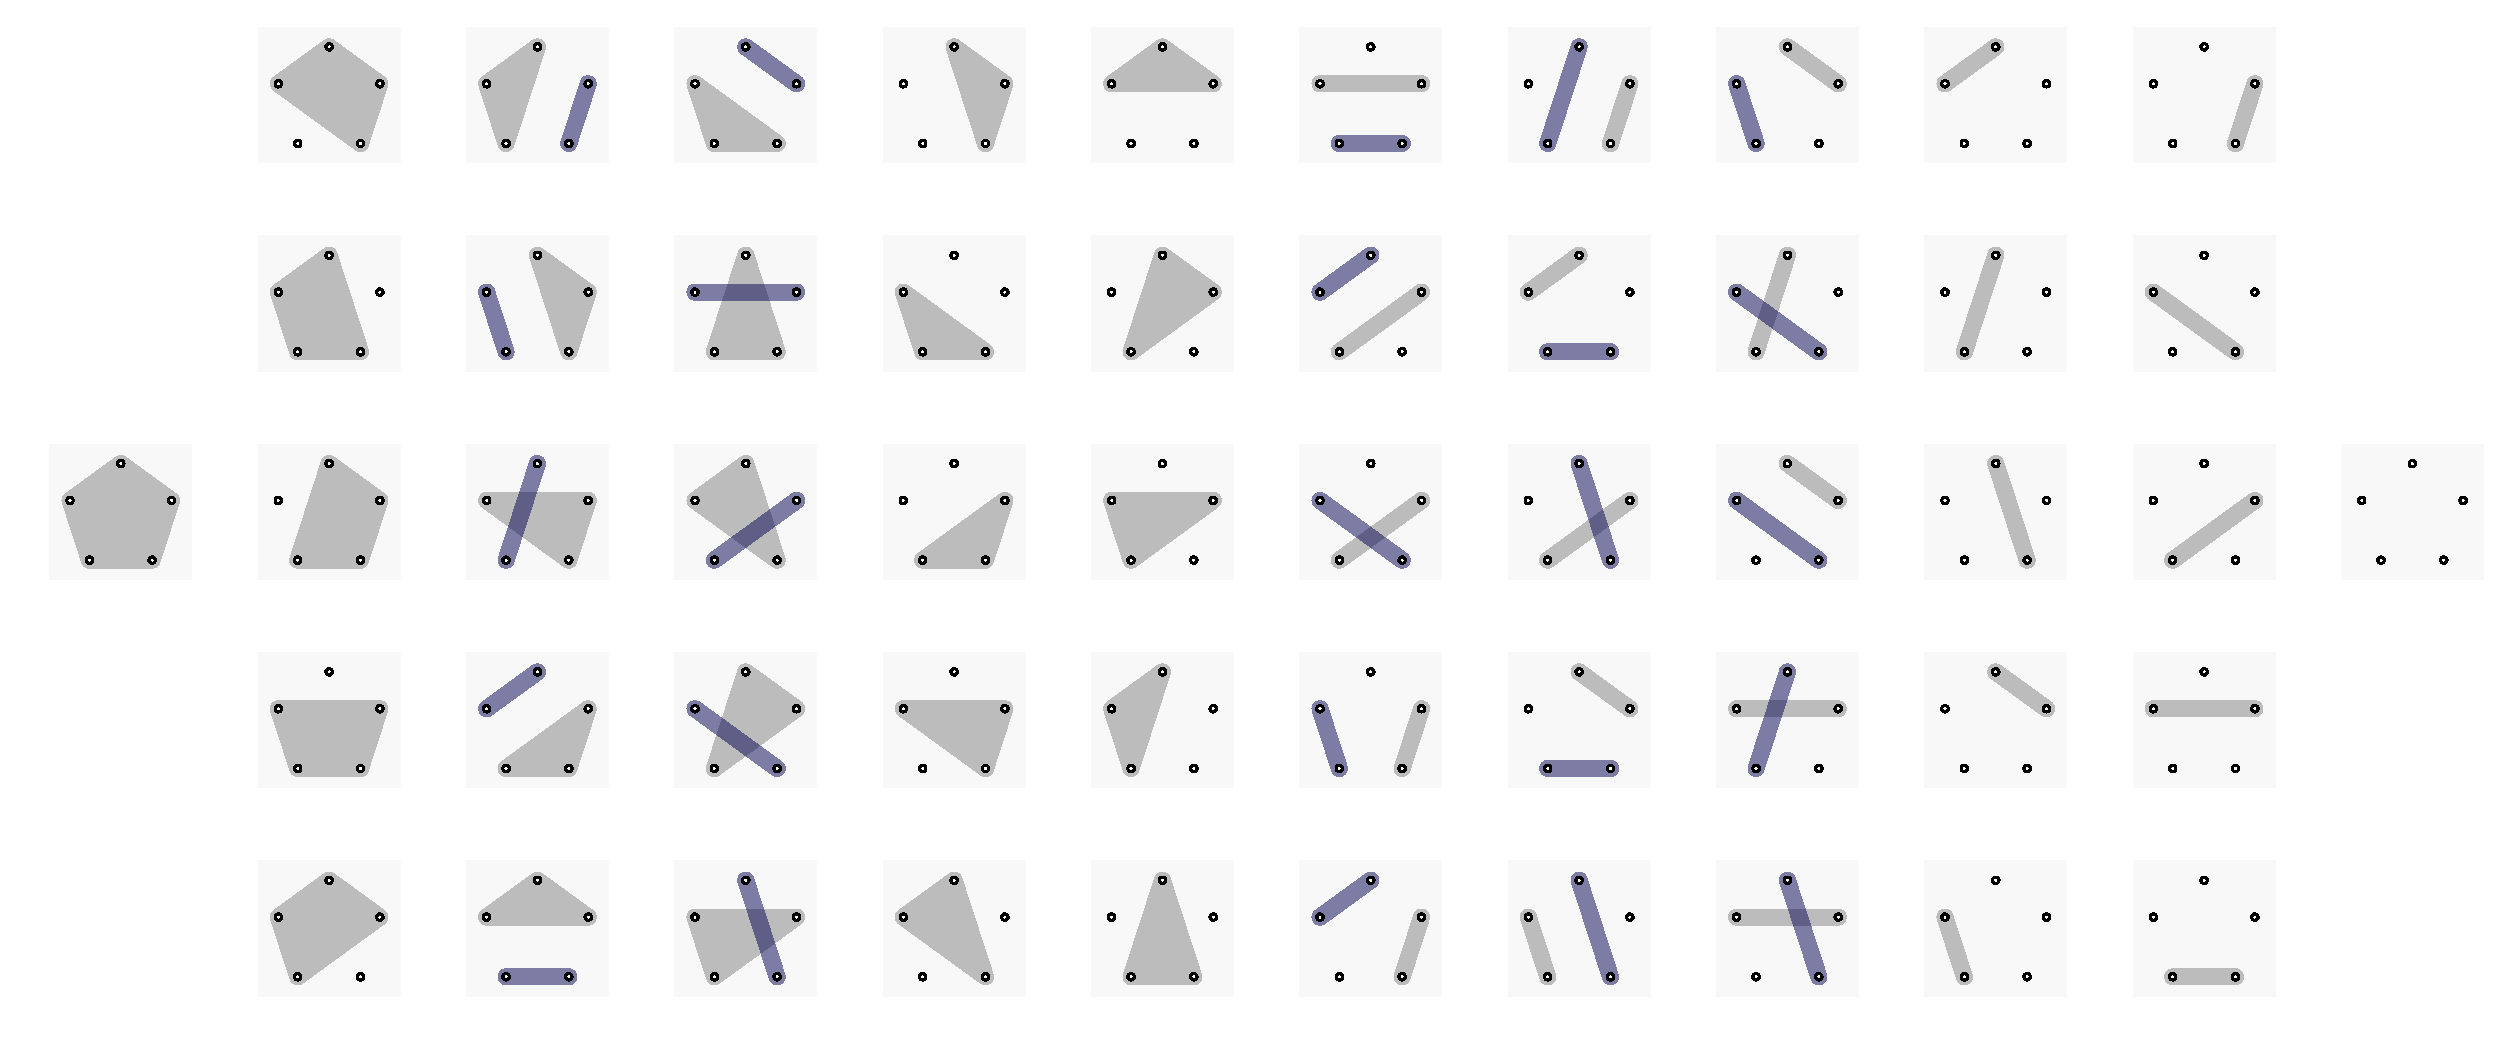
\includegraphics[width = \textwidth, keepaspectratio]{figures/modelspace_5_horizontal.pdf}
    \caption{All 52 possible models given $k = 5$, represented as partitions. Circles represent individual parameters and shaded regions indicate which parameters are equal.}
    \label{fig:partitions}
\end{figure}

The Stirling numbers and Bell numbers can be generalized to the $r$-Stirling \parencite{broder1984r} and $r$-Bell numbers \parencite{mezo2011r}, respectively. These generalizations help to construct conditional distributions, as we will see later. The $r$-Stirling numbers $\rstirling{k}{j}{r}$ give the number of partitions of size $j$ given $k$ parameters such that the first $r$ parameters are all in distinct subsets. The $r$-Bell numbers give the total number of partitions given $k$ parameters where the first $r$ parameters are in distinct subsets. Specifically, we have:
\begin{align}
    \rstirling{k}{j}{r} &= \sum_{i=0}^k \binom{k}{i}\stirling{i}{j}r^{k-i}\\
    \rbellnum{k}{r} &= \sum_{i=0}^k \rstirling{k+r}{i+r}{r} \enspace .
\end{align}
Note that $\rstirling{k}{j}{1} = \stirling{k}{j}$ and that $\rbellnum{k}{0} = \bellnum{k}$. Both the $r$-Stirling and $r$-Bell numbers are defined through recurrence relations, although explicit expressions exist which are easier to compute for large values; see \textcite{broder1984r} and \textcite{mezo2011r} for details.

\subsection{Urn Schemes}
We can represent the different partitions using an urn with $K$ different balls labeled 1 through $K$. For each parameter $\theta_j$, a ball $b_j$ is drawn from the urn with $b_j \in \{1, \ldots, K\}$. If two drawn balls are equal, $b_i = b_j$, then the two parameters are assigned to the same subset of the partition, that is, the two parameters $\theta_i$ and $\theta_j$ are equal if $b_i = b_j$. Note that different draws from an urn can represent the same partition. For example, the draws $(1, 1, 2)$ and $(3, 3, 1)$ both represent the partition $\{\{\theta_1, \theta_2\}, \{\theta_3\}\}$. The prior distributions introduced in the next sections assign probabilities to the unique partitions. Note that the prior probability of a particular draw can be obtained by dividing the probability of the corresponding partition by the total number of draws that correspond to that partition. The total number of draws that represent the same partition is given by $d!\binom{k}{d}$ where $d$ is the number of non-empty subsets of a particular draw.

% not sure how to bring this up
Although the urn consists of $K$ different balls, the event of interest is the whether the next ball drawn equals one of the balls already drawn --- in other words, whether an equality or inequality is introduced. This event reduces the urn to a P\'{o}lya urn. All prior distributions discussed below are related to the P\'{o}lya urn. Specifically, the joint prior distribution on $(\theta_1, \ldots, \theta_K)$ is characterized by a (generalized) P\'{o}lya urn such that:
\begin{equation} \label{eq:prediction-rule}
    P(\theta_K \mid \theta_1, \ldots, \theta_{K - 1}) = \begin{cases}
    \zeta_j & \text{with probability } P_{\pi} \\
    \theta_j^{\star} & \text{with probability }  1- P_{\pi} \enspace ,
    \end{cases} \numberthis
\end{equation}
where $\zeta_j$ denotes a new value for $\theta_K$ (with $\theta_1 = \zeta_1$) and $\theta_j^{\star}$ denotes a value equal to any previously observed value. We characterize the priors we discuss in the next section in terms of (\ref{eq:prediction-rule}), which is known as a \textit{prediction rule} \parencite[e.g.,][]{ishwaran2001gibbs}; in terms of the induced prior over partitions; and in terms of their penalty for multiplicity.

%\FD{\textcite{ishwaran2001gibbs} might be useful, they use Polya Urns to derive a Gibbs sampler. They say it can be used for the Dirichlet process, but also for \textit{any} prior with known \textit{prediction rule}, which is defined as $P(Y_{n+1} \mid Y_1, \ldots, Y_n)$. I think this is a useful description which allows us to distinguish between several priors (Dirichlet, Pittman-Yor, beta-binomial, etc.). Maybe note this here and then we refer to the next sections, in which we discuss the priors in slightly more detail?}
% We want to make inference over all possible partitions of some population parameter vector $\mathbf{\theta} = (\theta_1, \ldots, \theta_k)$ of size $k$. Each such partition corresponds do one particular hypothesis. The number of partitions $k$ is given by the Bell number

% \begin{equation}
%     B_{k + 1} = \sum_{i = 0}^k {k \choose i} B_k \enspace .
% \end{equation}

% The Bell numbers grow very quickly, with the number of partitions for a vector $\mathbf{\theta}$ of size 10 being 21147.


\section{Methodology} \label{sec:methodology}
Let $\vec{\theta^{\star}} = (\theta^{\star}_1, \ldots, \theta^{\star}_m)$ denote the vector of unique population parameters out of $\vec{\theta} = (\theta_1, \ldots, \theta_k)$ and denote the number of repeats of $\theta^{\star}_j$ as $n^{\star}_j$. Let $\rho$ denote a partition and $|\rho|$ its size. For example, if $\rho = \{\{\theta_1, \theta_2\}, \{\theta_3\}\}$, then $|\rho| = 2$. Similarly, for this example $\vec{\theta^{\star}} = (\theta^{\star}_1, \theta^{\star}_2)$ and $n^{\star} = (2, 1)$. In the next sections, we discuss and contrast a number of priors.

\subsection{Dirichlet Process Prior}
The Dirichlet process (DP) is a distribution over distributions \parencite{ferguson1973bayesian}. We say that $\mathcal{G} \sim \text{DP}(\alpha, \mathcal{K})$ is distributed according to a DP if its marginal distributions are Dirichlet distributed, where $\alpha$ is a concentration parameter and $\mathcal{K}$ is the base distribution; for details, see for example \textcite{teh2010dirichlet}. The DP can be understood as the infinite-dimensional generalization of the Dirichlet distribution \parencite[e.g.,][]{teh2010dirichlet}, which makes it popular for mixture modeling \parencite[e.g.,][]{rasmussen1999infinite}. Our modeling approach is similar to mixture modeling, except that we do not cluster data but parameters --- a cluster corresponds to a partition. Let $\vec{\theta}_{-j}$ be the vector of parameters without parameter $\theta_j$. The prediction rule of the DP is given by \parencite[e.g.,][]{ishwaran2001gibbs, blackwell1973ferguson}:
\begin{equation}
    \theta_j \mid \vec{\theta}_{-j} \sim \begin{cases}
    \mathcal{K} & \text{with probability } \frac{\alpha}{\alpha + j - 1} \\
    \text{Categorical}\left(\theta_1^{\star}, \ldots, \theta_m^{\star} \mid n^{\star}_1, \ldots, n^{\star}_m\right) & \text{else} \enspace ,
    \end{cases} \numberthis
\end{equation}
where $\alpha$ is the concentration parameter and the base distribution of the DP depends on the application (see Section \ref{sec:applications}). In other words, we draw a new value for $\theta_j$ from H with probability $\nicefrac{\alpha}{\alpha + j - 1}$, or else set it to a previously observed value. The particular value $\theta^{\star}_j$ the parameter $\theta_j$ is set to is proportional to the number of times $\theta^{\star}_j$ was observed previously, given by $n^{\star}_j$, resulting in the well-known ``rich-get-richer'' property \parencite[e.g.,][]{teh2010dirichlet}.

The Dirichlet process implies a prior distribution over partitions --- the so-called \textit{Chinese Restaurant Process} \parencite[e.g.,][]{teh2010dirichlet}. The prior on the partitions $\rho$ is:
\begin{equation}
    \pi(\rho \mid \alpha) = \frac{\alpha^{|\rho|}\Gamma(\alpha)}{\Gamma(n + \alpha)} \prod_{c \in \rho} \Gamma(|c|) \enspace ,
\end{equation}
where $c$ is an element of $\rho$, and $|c|$ is its size. While the Dirichlet process features the infinite-dimensional object $\mathcal{G}$, the prior over partitions results from integrating it out. Hence the nonparametric model (in which the number of parameters is not fixed) implies a parametric model (in which the number of parameters is fixed) for the partitions \parencite{quintana2006predictive}. This makes it usable for our purposes, where we have a fixed number of parameters.

The leftmost column in Figure \ref{fig:prior-comparison} shows the DP prior over partitions (top) and number of inequalities (bottom) for different values of $\alpha$. The value suggested by \textcite{gopalan1998bayesian} (in the $K = 5$ case, $\alpha = \nicefrac{5}{3}$) creates a symmetric prior over the partitions (green line). Only values $\alpha < 1$ result in a monotonically decreasing prior probability for an increasing partition size, which corresponds to a monotonically decreasing prior probability for an increasing number of inequalities (orange line). A requirement for a prior to penalizes multiplicity is to be monotonically decreasing with the number of partitions. If this were not the case, then models with many partitions, that is, many inequalities among parameters, would be more likely than models with few partitions, that is, few inequalities among parameters.

As $\alpha \rightarrow 0$, the prior of the model with all $K - 1$ equalities $\mathcal{M}_0$ converges to one, while as $\alpha \rightarrow \infty$, the prior of the model with $K - 1$ inequalities $\mathcal{M}_{B_k}$ converges to one. For prior elicitation, \textcite{gopalan1998bayesian} note that $\alpha$ is determined by specifying two of either $P(\mathcal{M}_0)$, $P(\mathcal{M}_{B_k})$, or their ratio, since $P(\mathcal{M}_0) = \nicefrac{\alpha (K - 1)!}{\prod_{j = 1}^K (\alpha + j - 1)}$ and $P(\mathcal{M}_{B_k}) = \nicefrac{\alpha^K}{\prod_{j = 1}^K (\alpha + j - 1)}$.

%\textcite{escobar1995bayesian} put a Gamma prior on $\alpha$.

\begin{figure}
    \centering
    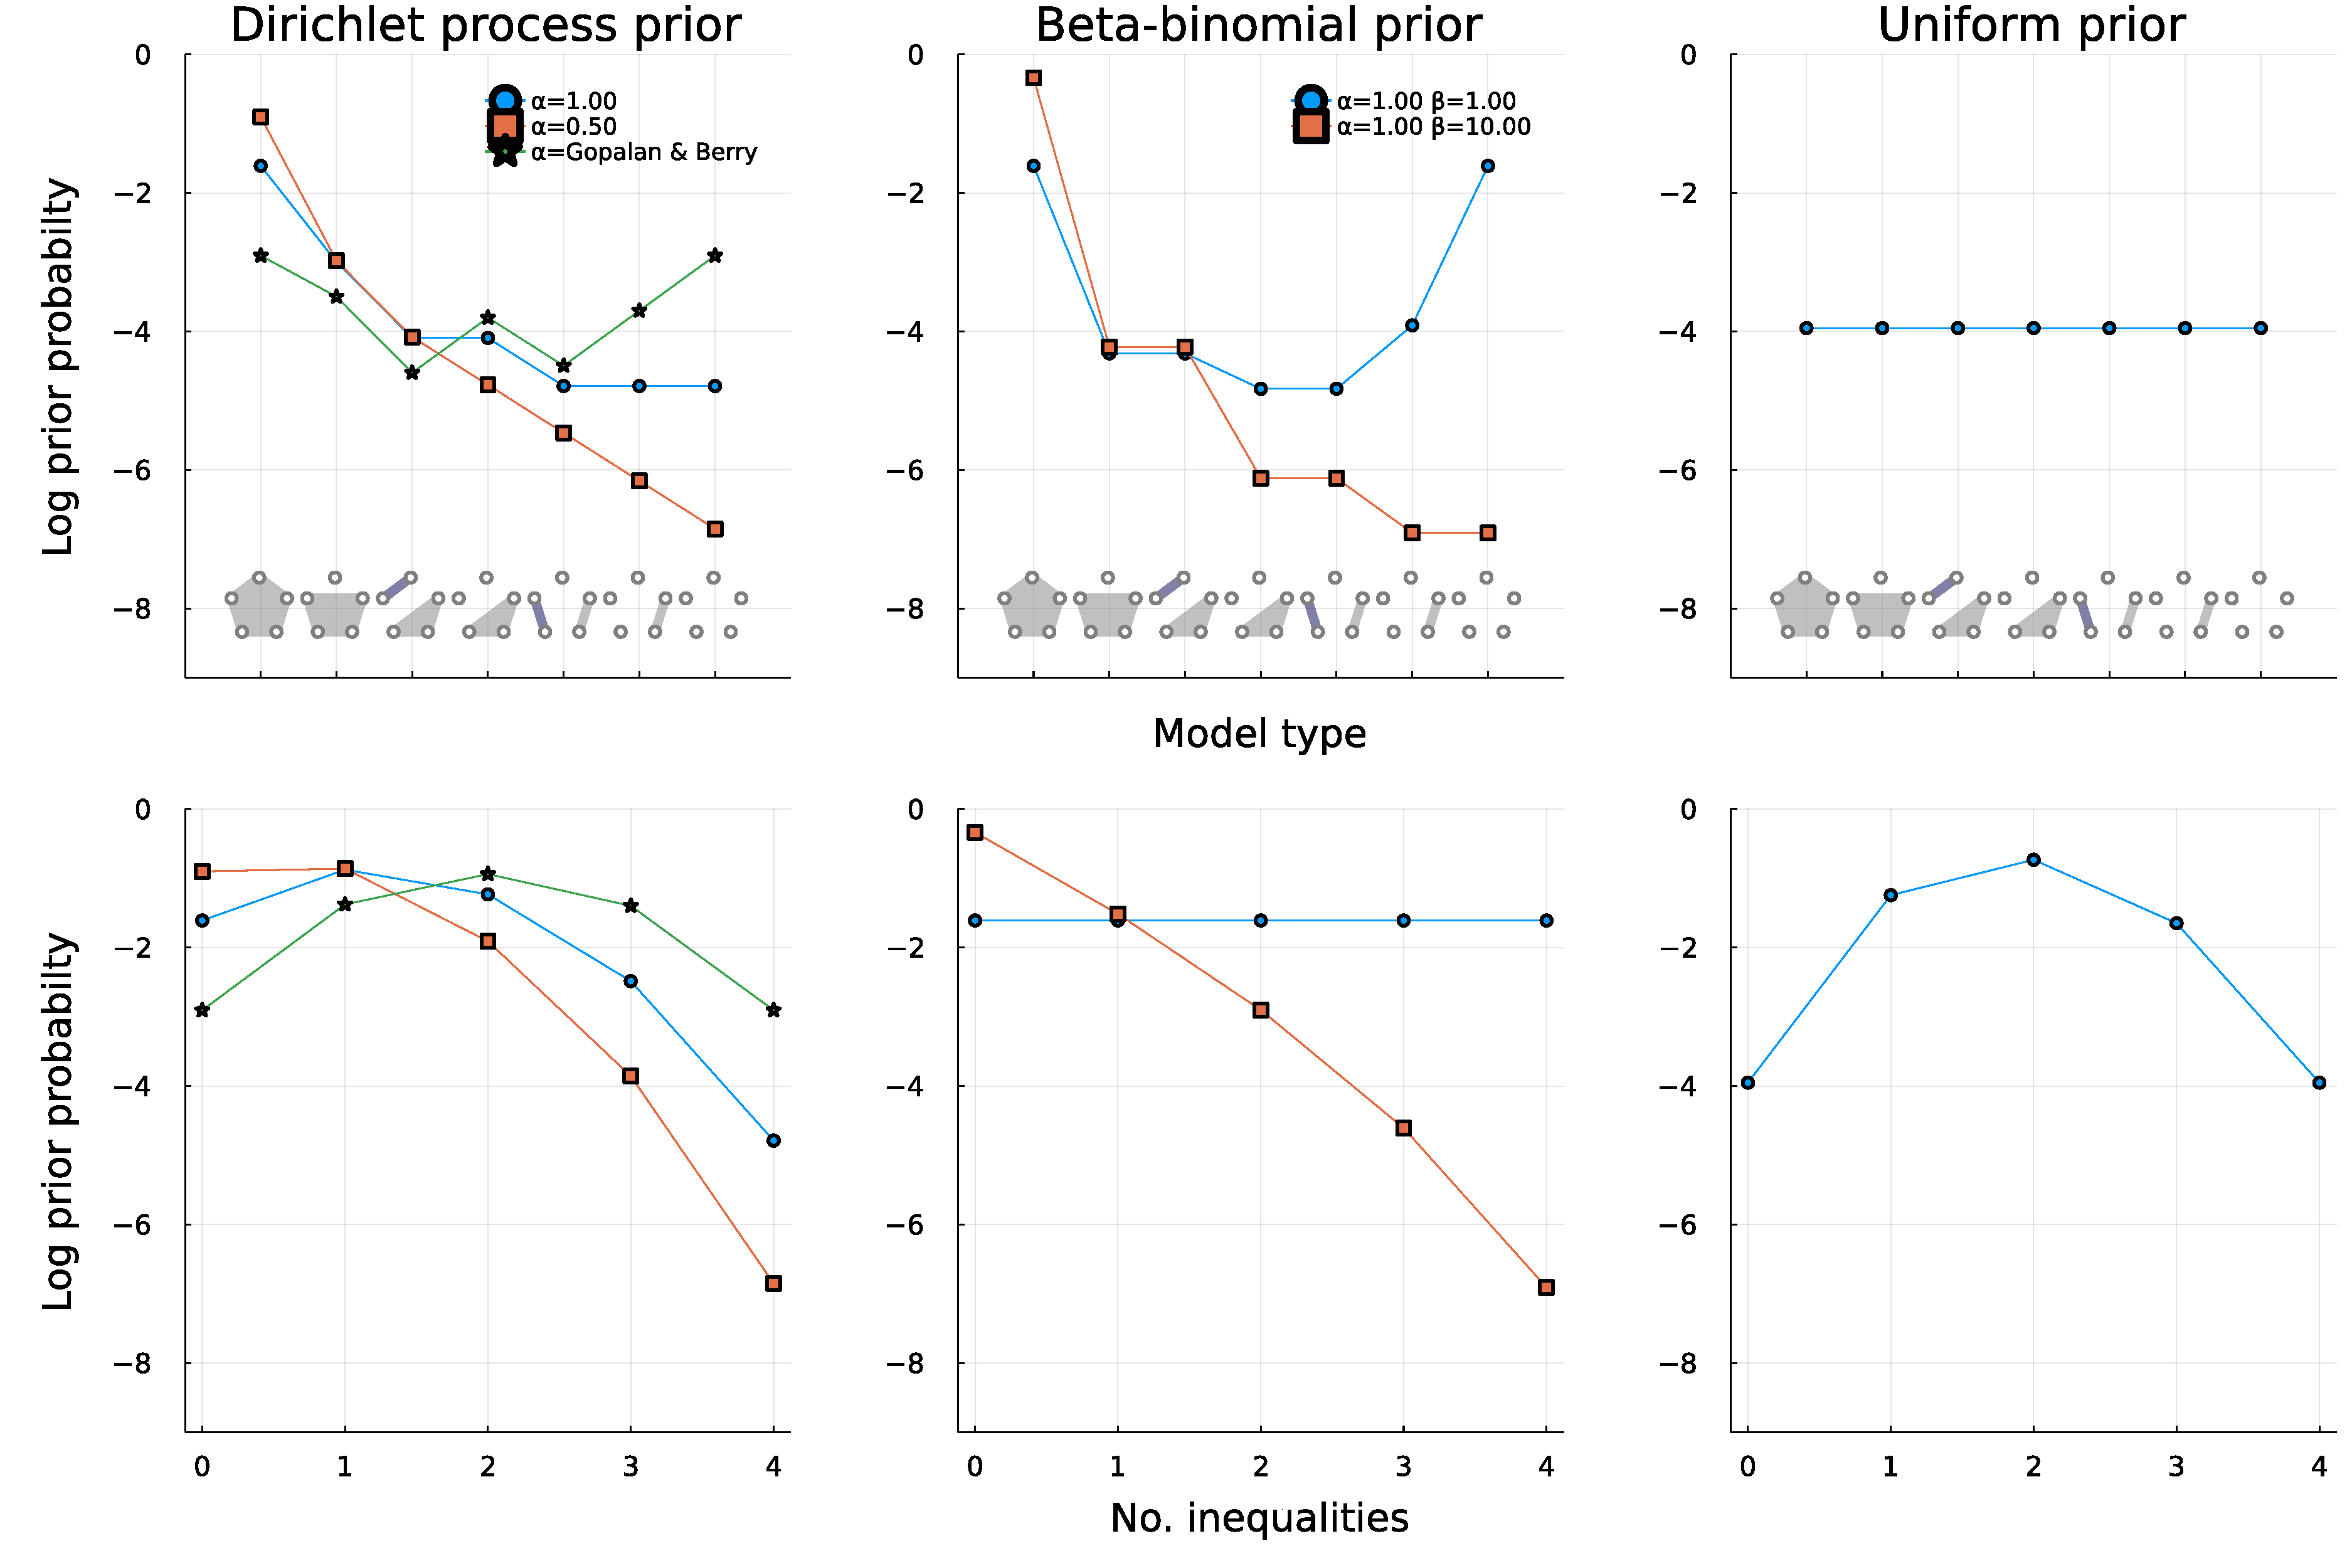
\includegraphics[width = 0.95\textwidth]{figures/visualizePriors_2x3.pdf}
    \caption{Top: Dirichlet process (left), beta-binomial (middle), and uniform prior (right) across distinct model types for $K = 5$ groups and different prior parameters. Bottom: Same but for the number of inequalities across models.} %Note that while the uniform prior is uniform over the models, it is not uniform over the number of inequalities. In contrast, the beta-binomial prior with $\alpha = \beta = 1$ is uniform over the number of inequalities but not uniform over the models.} %A key difference between the Dirichlet and beta-binomial priors is that the second and third partition, which imply the same number of equality constraints, are assigned equal prior probability by latter but not the former.}
    \label{fig:prior-comparison}
\end{figure}


\subsection{Beta-binomial Prior}
%Here we briefly introduce the beta-binomial model prior, its properties, and how we can apply use it to the space of equality constraints.

The beta-binomial model prior is a popular choice for stochastic search variable selection in linear regression \parencite[][]{george1993variable} or Bayesian model averaging \parencite[e.g.,][]{hinne2020conceptual, hoeting1999bayesian}. It states that the prior probability of including $j$ predictors out of a total of $K$ predictors is given by
\begin{equation}
    \BetaBinom{j}{K}{\alpha}{\beta} = \binom{K}{j} \frac{\FBeta{j + \alpha}{K - j + \beta}}{\FBeta{\alpha}{\beta}} \enspace ,
\end{equation}
where $\alpha$ and $\beta$ are hyperparameters. The prior probability of a particular model is obtained by dividing by the number of ways $j$ out of $K$ predictors can be included: $\BetaBinom{j}{K}{\alpha}{\beta} / \binom{K}{j}$. The advantage of the beta-binomial distribution is that it introduces a penalty for including additional predictors and in that way introduces a correction for multiplicity \parencite{scott2006exploration, scott2010bayes}.

In the space of equality constraints, we consider the number of inequality constraints and use the beta-binomial prior to introduce a penalty for each additional inequality among the groups considered. This results in a $\BetaBinom{j}{K-1}{\alpha}{\beta}$ prior distribution over the number of included inequalities $j$ out of $K$ groups. The number of ways one can choose $j$ out of $K-1$ inequalities is equivalent to the Stirling number $\stirling{K}{K-j}$, which counts how many partitions of size $K - j$ there are out of the $K$ groups. Thus the prior probability for a particular model is given by $\BetaBinom{j}{K-1}{\alpha}{\beta} / \stirling{K}{K-j}$. The prediction rule of the beta-binomial prior is given by:
\begin{equation}
    \theta_j \mid \vec{\theta}_{-j} \sim \begin{cases}
    \mathcal{K} & \text{with probability } P_{\pi} \\
    \text{Categorical}\left(\theta_1^{\star}, \ldots, \theta_m^{\star} \mid \rbellnum{K - 1 - 1}{s_1}, \ldots, \rbellnum{K - m - 1}{s_m}\right) & \text{else} \enspace .
    \end{cases} \enspace , \numberthis
\end{equation}
where
\begin{equation}
    P_{\pi} = \frac{
        \sum_{i=1}^K \BetaBinom{i}{K}{\alpha}{\beta} \rstirling{K-i-s_j-1}{K-i+1}{s_j + 1}
    }{
        s_j \sum_{j=i}^K \BetaBinom{i}{K}{\alpha}{\beta} \rstirling{K-i-s_j-2}{K-i+1}{s_j} +
          \sum_{i=1}^K \BetaBinom{i}{K}{\alpha}{\beta} \rstirling{K-i-s_j-1}{K-i+1}{s_j + 1}
    } \enspace ,
\end{equation}
where $s_j = \setsize{\{\theta_1, \ldots, \theta_{j - 1}\}}$ is the number of distinct elements in $\{\theta_1, \ldots, \theta_{j - 1}\}$. The $r$-Stirling number in the numerator counts the number of models with $i$ equalities if $\theta_j$ is a new value. Next, this is multiplied by the probability of including $i$ equalities. This is summed for all possible numbers of equalities. 
The first sum in the denominator does the same, assuming that $\theta_j$ is a value in $\{\theta_1, \dots, \theta_{j-1}\}$. With probability $1 - P_{\pi}$ we have that $\theta_j$ is equal to one of the previously drawn parameters. This draw is from a categorical distribution over the possible models, that is, conditional on drawing a previous value the probability of $\theta_j = \theta_i$ is proportional to $\rbellnum{K-i-1}{s_j}$. \FD{Double check this and adjust the text and Equation (9).}

The beta-binomial prior on the partitions and the induced prior on the number of inequalities are shown for different parameterizations in the middle column in Figure \ref{fig:prior-comparison}. The standard parameterization of the beta-binomial distribution has a characteristic U-shape that, if not apparent for a fixed number of groups $K$, will become apparent as $K$ is increased. We follow \textcite{wilson2010bayesian} who, in the context of regression, suggested to set $\alpha = 1$ as a default so that the distribution on model size is nonincreasing, and to scale $\beta = \lambda K$ with the number of groups ($\beta = \lambda K$) to force the prior to be monotonically decreasing, with a default of $\lambda = 1$ \parencite{wilson2010bayesian}. The difference is that in our prior specification the roles of $\alpha$ and $\beta$ are reversed. This specification leads to a penalty for multiplicity, as the orange line in Figure \ref{fig:prior-comparison} shows. Setting $\alpha = 1$ would instead result in a uniform prior over the number of inequalities (blue line), and no penalty for multiplicity.

Figure \ref{fig:prior-comparison} shows that the DP prior makes a distinction that the beta-binomial is, by design, not making: while the beta-binomial prior assigns the same prior mass to partitions with the same number of (in)equalities, the DP prior assigns more mass to the partition with the larger cluster. For example, the beta-binomial does not distinguish between $\{\{\theta_1, \theta_2, \theta_3\}, \theta_4, \theta_5\}$ and $\{\{\theta_1, \theta_2\}, \{\theta_3, \theta_4\}, \theta_5\}$, while the DP assigns more mass to the former (see Figure \ref{fig:prior-comparison}). We return to this distinction in the discussion.

\subsection{Uniform Prior}
%\FD{The paper by \textcite{wallach2010alternative} seems extremely relevant here. The define the uniform process as having a prediction rule that is uniform over the already existing partitions ... so not quite the same. How is it related to what we do here? Actually, they show that the expected number of clusters of size $M$ is a constant, so it seems to be exactly what we do. Interestingly, the uniform process is not exchangeable. Also, it seems to me that it will not penalize multiplicity.}
For completeness, we give a prior that is uniform over the space of partitions. The probability mass function is straightforward. All valid configurations of size $K$ have probability $\nicefrac{1}{\bellnum{K}}$. The prediction rule of the uniform prior is given by:
\begin{equation}
    \theta_j \mid \vec{\theta}_{\backslash j}%, \ldots, \theta_{j - 1}, \theta_{j + 1}, \ldots, \theta_{K} 
    \sim \begin{cases}
    \mathcal{K} & \text{with probability } \rbellnum{K - j - 1}{s_j + 1} \\
    \text{Categorical}\left(\theta_1^{\star}, \ldots, \theta_m^{\star} \mid \rbellnum{K - 1 - 1}{s_1}, \ldots, \rbellnum{K - m - 1}{s_m}\right) & \text{else} \enspace ,
    \end{cases} \numberthis
\end{equation}
For the first value $\theta_1$, the drawn value is irrelevant as it does not introduce an (in)equality. For the second draw we consider two cases. First, the probability of drawing a new value $\theta_2 \neq \theta_1$ is proportional to the number of partitions where the first two elements are in distinct subsets, which is given by $\rbellnum{K - 2}{2}$. The probability of sampling a particular new value is uniformly divided over the possible labels; hence to obtain the probability for a particular new value we divide by $K - s_j$. \FD{I don't understand the previous sentence, let's discuss.} Second, the probability of drawing an old label, $\theta_2 = \theta_1$, is proportional to the number of partitions where the first element is in a distinct subset. Under this uniform prior, all partitions $\rho$ are equally likely, as can be seen in the top right panel in Figure \ref{fig:prior-comparison}. Note that this uniform prior induces a non-uniform prior on the number of inequalities, as shown in the bottom right panel.

\iffalse
\begin{equation}
    \prior{\theta_i \mid \theta_1, \ldots, \theta_{i - 1}} = \begin{cases}
    \zeta_i & \text{with probability proportional to } \rbellnum{k - i - 1}{s_i + 1} \\
    \theta_i^\ast & \text{with probability proportional to }  \rbellnum{k - i - 1}{s_i} \enspace
    \end{cases} \numberthis
\end{equation}
\fi

\subsection{Posterior Model Consistency}
Model selection consistency is a key desiderata that a good Bayes factor should fulfill \parencite[e.g.,][]{bayarri2012criteria, ly2016harold, consonni2018prior}. In the situation of multiple models, the notion of pairwise model selection consistency needs to be extended. This is referred to as posterior model selection consistency. Posterior model consistency in a model class $\mathfrak{M}$ is the convergence to one, in probability, of the posterior probabilities to the true model \parencite[e.g.,][]{casella2009consistency, moreno2015posterior}. Let $\mathcal{M}_j \in \mathfrak{M}$ be the model that instantiates the hypothesis $\mathcal{H}_j$ that specifies the (in)equalities among $K$ groups. The posterior probability of $\mathcal{M}_j$ is given by:
\begin{align}
    p(\mathcal{M}_j \mid \mathcal{D}) &= \frac{p(\mathcal{D} \mid \mathcal{M}_j) \pi(\mathcal{M}_j)}{\sum_{i = 0}^{\bellnum{K}} p(\mathcal{D} \mid \mathcal{M}_i) \pi(\mathcal{M}_i)} 
    = \frac{\text{BF}_{j0}\pi(\mathcal{M}_j)}{\sum_{i = 0}^{\bellnum{K}} \text{BF}_{i0} \pi(\mathcal{M}_i)} \enspace .
\end{align}
It follows that if the Bayes factor is model selection consistent, posterior model consistency holds \parencite[see also][Theorem 1]{moreno2015posterior} --- unless the prior assigns zero mass to the true model. This is not the case for any of the priors discussed above, and hence whether posterior model consistency holds depends solely on the priors on the parameters within models.

\subsection{Stochastic Search Method} \label{sec:method-description}
When the number of groups is small and the computation of Bayes factors is swift, one can directly compute the Bayes factors for all hypotheses. Using the priors we outlined above, one can then obtain posterior distributions over hypotheses that incorporate the desired multiplicity adjustment. The number of (in)equalities grows extremely quickly with the number of groups, however, and for larger number of groups one must rely on stochastic search methods. Moreover, while directly computing the Bayes factors results in posterior distributions over hypotheses, it does not yield posterior distributions over parameters. We therefore setup a stochastic search method that yields both, allowing researchers to incorporate uncertainty across hypotheses through model averaging \parencite[e.g.,][]{hinne2020conceptual, hoeting1999bayesian}.

Our method is implemented in the programming language Julia \parencite{Julia2017Bezanson}. First, we implemented the prior distributions in Julia. Next, we used the library \emph{Turing.jl} which is designed for general-purpose probabilistic programming \parencite{Turing2018Ge}. Turing enabled us to directly reuse the distributions defined in Julia code and also provided a multitude of options for composing different MCMC samplers. We set up a Gibbs sampler that explored the posterior space in two steps. The first step used Turing's built in Hamiltonian Monte Carlo methods for sampling from the posterior distributions of the continuous parameters. In all models discussed here, all parameters are continuous except for the partitions. The second step used a custom Gibbs algorithm for sampling from the posterior distribution over partitions. The partitions were represented as a vector of integers denoted $\vec{\gamma}$ that indicate partition membership. By partition membership we mean that two parameters $\theta_i$ and $\theta_j$ are in the same partition if and only if $\gamma_i = \gamma_j$. For example, $\{\{\theta_1\}, \{\theta_2, \theta_3\}\}$ could be represented by $(1, 2, 2)$ but also by $(3, 1, 1)$. We first explain the remainder of the sampling scheme and motivate the duplicate representations in the next paragraph. The number of possible duplicate representations in $\vec{\gamma}$ for one partition is straightforward to compute, and the prior over $\vec{\gamma}$ is obtained by taking the prior over the partitions and dividing uniformly over duplicate representations. Next, we sample each element of $\vec{\gamma}$ conditional on the other elements. Since the partition membership is discrete, we enumerate all possible values and draw from the resulting categorical distribution. Sampling individual elements of $\vec{\gamma}$ from the conditional distributions rather than the joint distribution reduces the complexity from $\mathcal{O}(B_K)$ to $\mathcal{O}(K^2)$.

Although the duplicate representations of $\vec{\gamma}$ for one partition introduce some additional computational cost, they facilitate exploration of the posterior space. For example, had we used a one-to-one mapping from partitions to $\vec{\gamma}$, then updating the first membership in $(1, 2, 2)$ to $(2, 2, 2)$ would not be a valid configuration, as this should be represented by $(1, 1, 1)$. However, a transition from $(1, 2, 2)$ to $(1, 1, 1)$ requires updating two parameters and is simply less likely to occur. Nevertheless, on the level of partitions, it makes sense to propose to move from $\{\{\theta_1\}, \{\theta_2, \theta_3\}\}$ to $\{\{\theta_1, \theta_2, \theta_3\}\}$.


\section{Investigating Multiplicity Adjustment} \label{sec:simulation-study}
In this section, we investigate the differences between the above priors in more detail. In Section \ref{sec:scott-berger}, we use a visualization inspired by \textcite{scott2010bayes} to illustrate the extent to which different priors penalize multiplicity. In Section \ref{sec:illustration}, we use a small simulation study to illustrate the implications of multiplicity adjustment. In Section \ref{sec:simulation}, we present the results of a more extensive simulation study comparing the three priors.

\subsection{Prior Comparison} \label{sec:scott-berger}
Figure~\ref{fig:scott_berger} illustrates the penalty imposed by the priors for including an additional inequality constraints into a model. The panels in the top row show the (log) prior probability of a model with a specific number of inequalities for a fixed number of groups $K = 30$ across the different priors. For the Dirichlet process prior, the prior probability is not uniquely determined by the number of inequality constraints (as illustrated in Figure~\ref{fig:prior-comparison}) and we therefore show the average prior probability of a model with a particular number of inequality constraints. As above, we see that the DP with $\alpha < 1$ and the beta-binomial prior with $\alpha = K$ show a monotonically decreasing trend as the number of inequality increases, while the uniform prior assigns equal prior mass to the models.

The panels in the bottom row show the prior odds of including additional inequality constraints as a function of how many inequalities are already present and the number of groups $K$. For example, the blue line shows the prior odds of going from a model with no inequalities ($P(\#0)$) to a model with one inequality ($P(\#1)$). For the DP prior (left), these prior odds are $1 / \alpha = 2$ in favour of the model with no inequalities across all group sizes $K$. For the beta-binomial prior, on the other hand, the prior odds in favour of the null model increase linearly with the number of groups; for $K = 1$, the prior odds are XXX, while for $K = 17$ they are XXX. The uniform prior gives equal prior odds across all group sizes. Note that the prior odds correspond to the exponentiated difference between the log prior values at 0 and 1 in the top panels.

While the blue line shows the prior odds of going from the null model to a model with one inequality, the orange line shows the prior odds of going from a model with one inequality to one with two inequalities, the green line from going from one with four to one with five, and the purple line from going to nine to one with ten. We see that, as the number of already existing inequalities increases, the penalty for including an additional one decreases. This is also encoded in the top panels, which for the DP and the beta-binomial prior show a less steep decrease as the number of inequalities increases.

\begin{figure}
    \centering
    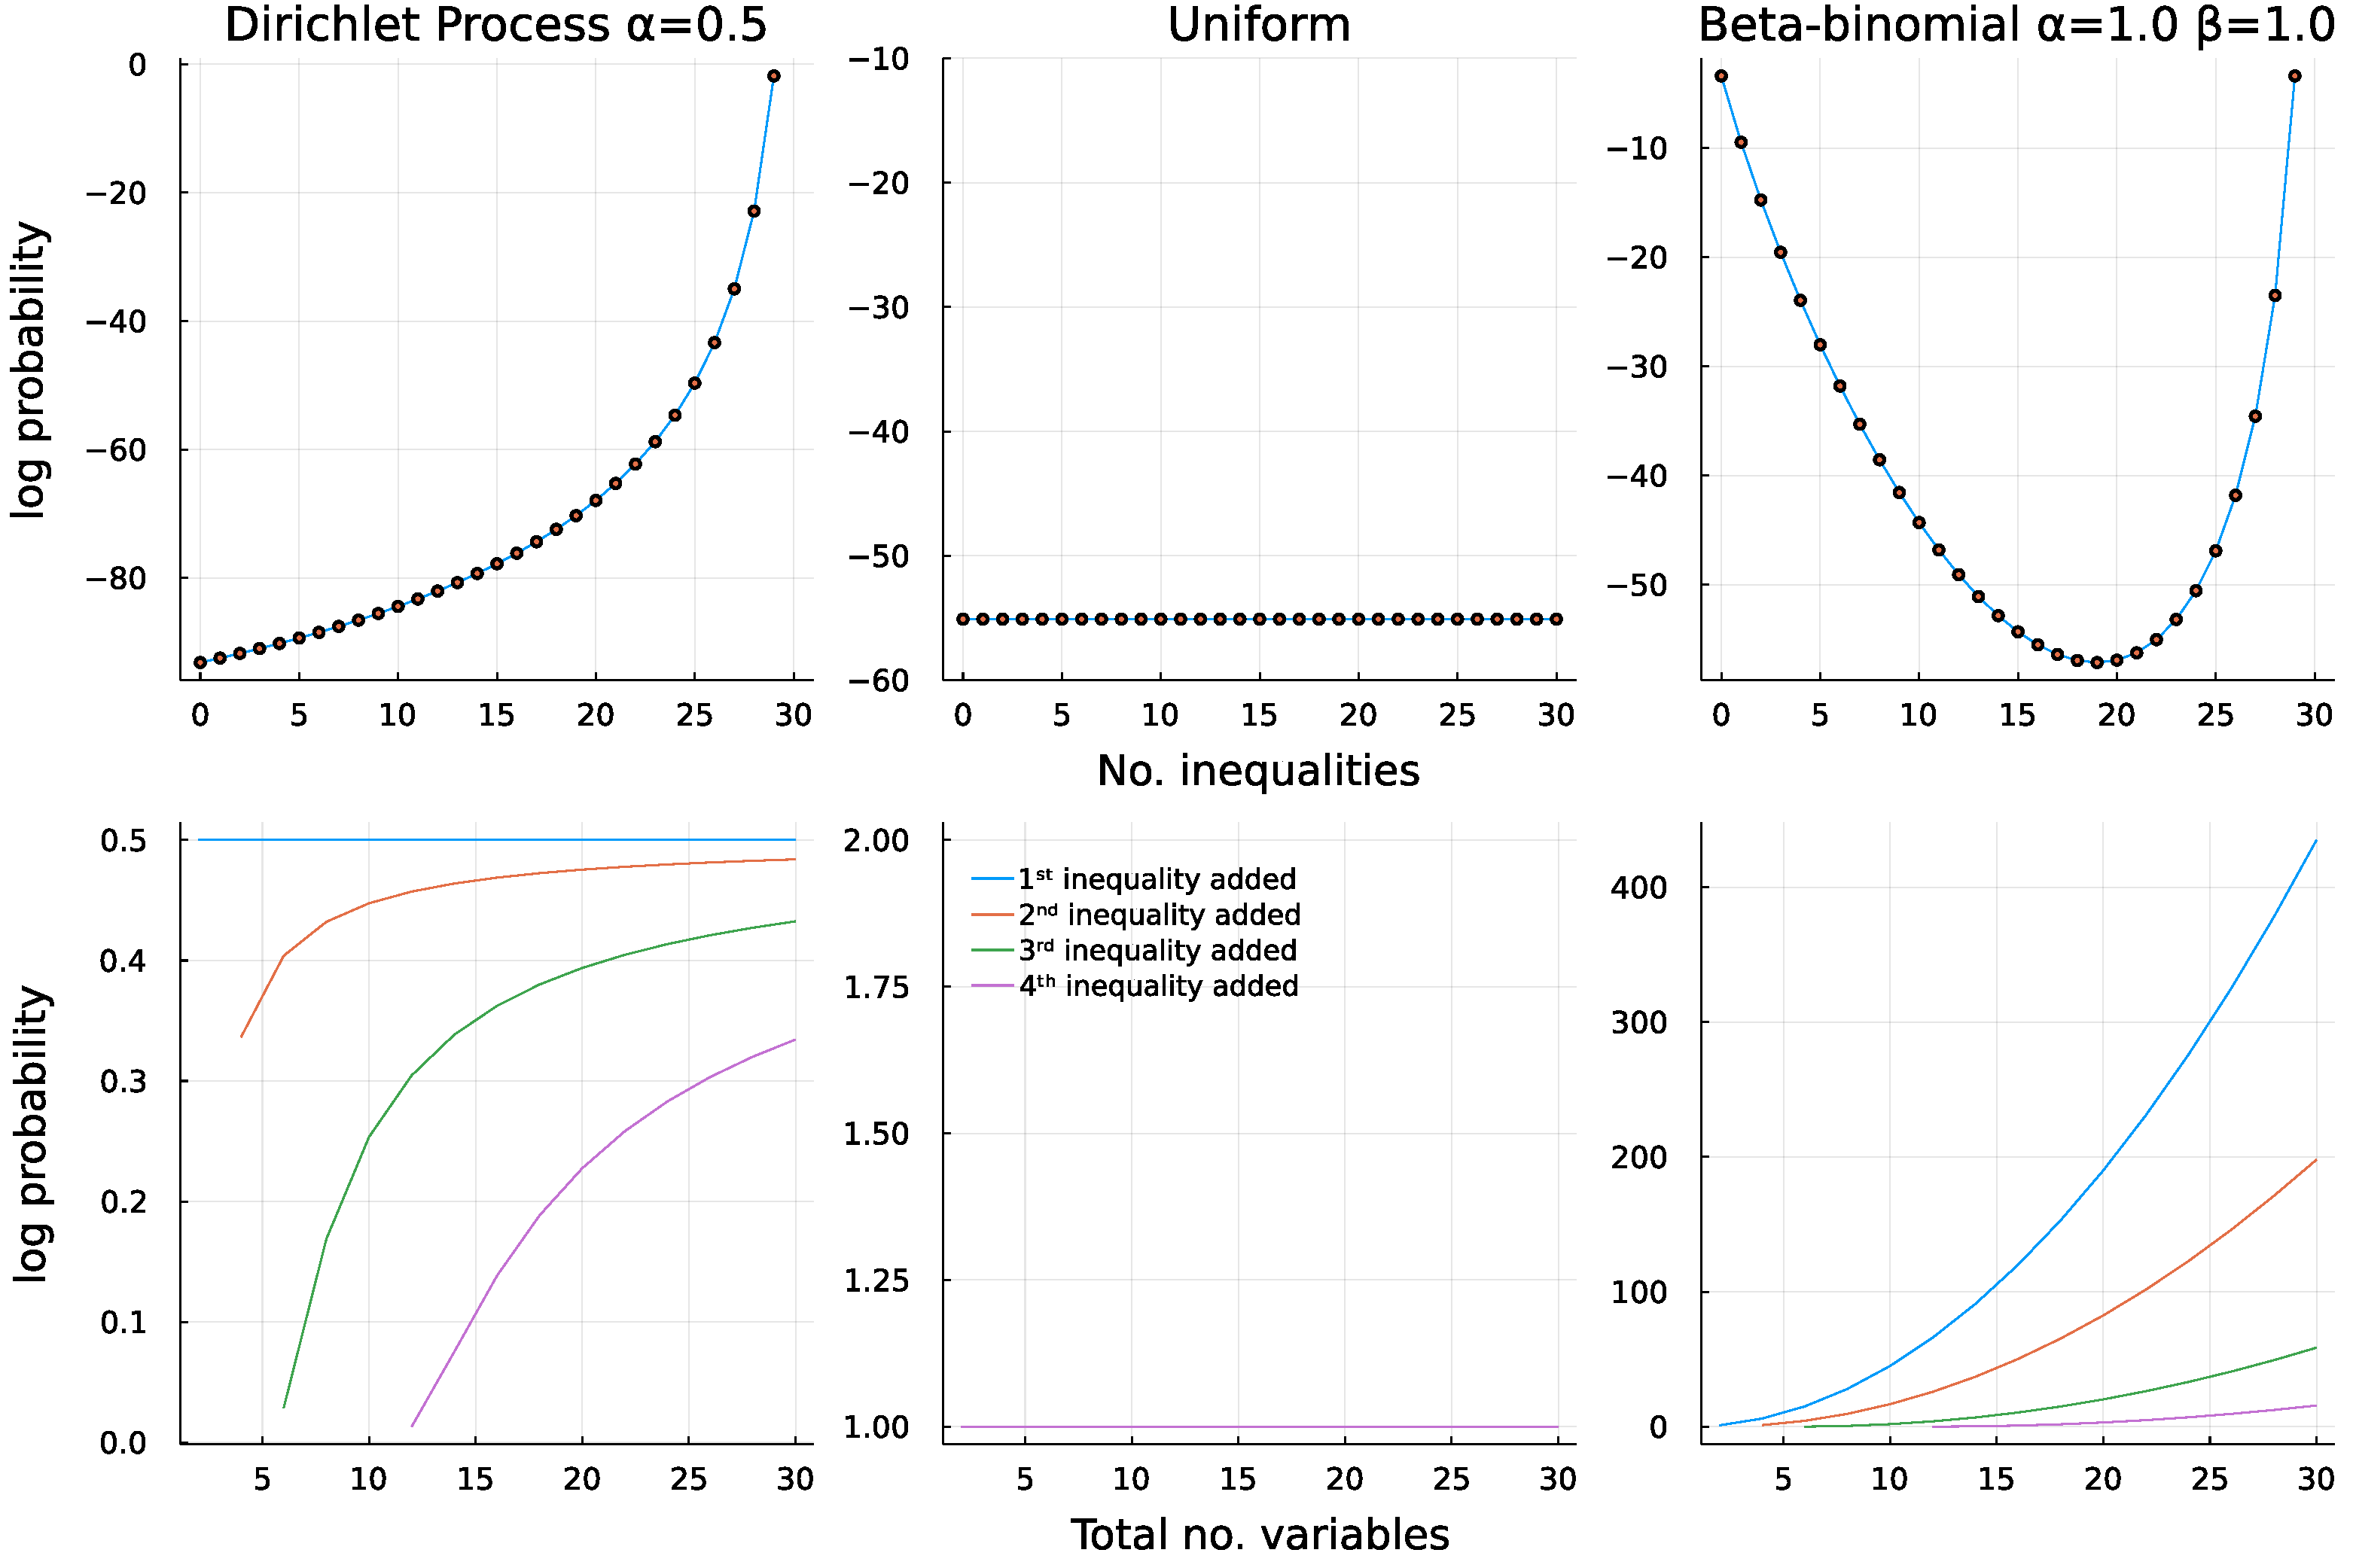
\includegraphics[width=0.89\textwidth]{figures/prior_comparison_plot_2x4_without_log_without_betabinomial.pdf}
    \caption{Top: Penalty imposed by the Dirichlet process, uniform, and beta-binomial priors for including additional inequality constraints. Shows log prior probability of the number of inequalities in the model for $K = 30$. Bottom: Shows the prior odds of adding one additional inequality to a model as a function of how many inequalities already exist (0: blue, 1: orange, 4: green, 9: purple) as a function of the number of groups $K$.}
    \label{fig:scott_berger}
\end{figure}

\subsection{Illustrating Multiplicity Adjustment} \label{sec:illustration}
Here we illustrate the different multiplicity penalties that the different priors impose using a small simulation study. We simulate data from a one-way ANOVA model and analyze it using the specification by \textcite{rouder2012default}. The data generating model is as follows:
\begin{align*}
    Y_{ij}              &\sim \mathcal{N}\left(\mu + \sigma\theta_j, \sigma^2\right)\\
    \mu                 &\sim \mathcal{N}\left(0, 1\right)  \\
    \sigma^2            &\sim \mathcal{IG}\left(1, 1\right) \\
    g                   &\sim \mathcal{IG}\left(\nicefrac{1}{2}, \nicefrac{1}{2}\right) \\
    \vec{\theta}^u   &\sim \mathcal{N}_{K-1}\left(0, g\right)   \\
    \vec{\theta}^c   &\leftarrow \mathbf{Q}\vec{\theta}^u \\
    \theta_j            &\leftarrow \text{mean of elements of } \theta^c \text{ in the same partition }\\
    \rho                &\sim \pi(.) \enspace . \numberthis
\end{align*}
The data are normally distributed with a grand mean $\mu$, a group specific offset $\theta_j$, and a variance $\sigma^2$. The offsets sum to zero to avoid identification constraints. This is achieved by projecting $\vec{\theta}^u$ from a $K-1$ dimensional space onto a $K$ dimensional space using the matrix $Q$, which consists of the first $K-1$ columns of an eigendecomposition of a degenerate covariance matrix as defined in \textcite{rouder2012default}.\footnote{Note that this projection is not unique. It can also be achieved with, for example, a QR decomposition, as recommended by the \textcite{stanUserManual}.} Next, the elements of $\vec{\theta}^c$ within the same partition are averaged to obtain $\theta_j$. The unconstrained offsets $\vec{\theta}^u$ are assigned a $g$ prior where $g$ itself is assigned an inverse gamma prior with shape and scale equal to \nicefrac{1}{2} \parencite{liang2008mixtures}. Note that the model reduces to the approach of \textcite{rouder2012default} whenever the partition indicates that all elements are distinct.

We simulated from the null model which assumes that all the groups are equal, drawing 100 observations per group and varying the number of groups $K \in [2, 3, \dots, 10]$, repeating each combination 100 times. For the analysis we considered six priors: the Dirichlet process prior (DPP) with $\alpha = 0.50$, $\alpha = 1$, and $\alpha$ set adaptively to have equal prior mass assigned to the model with all equalities and the model with all inequalities (i.e., $p(\mathcal{H}_0) = p(\mathcal{H}_1)$), as done by \textcite{gopalan1998bayesian}; the beta-binomial prior with $\alpha = K , \, \beta = 1$ and $\alpha = 1, \, \beta = 1$; and the uniform prior. We used our methodology as described in Section \ref{sec:method-description}, drawing 12,000 MCMC samples and discarding the first 2,000 as a burn-in.

To assess how well the respective priors adjust for multiplicity, we calculated how frequently the posterior probability that any two groups differ is larger than 0.50, noting that the true model assumes that all groups are equal. Figure~\ref{fig:small_simulation} shows the probability of making one or more such errors as a function of the number of groups.
\begin{figure}
    \centering
    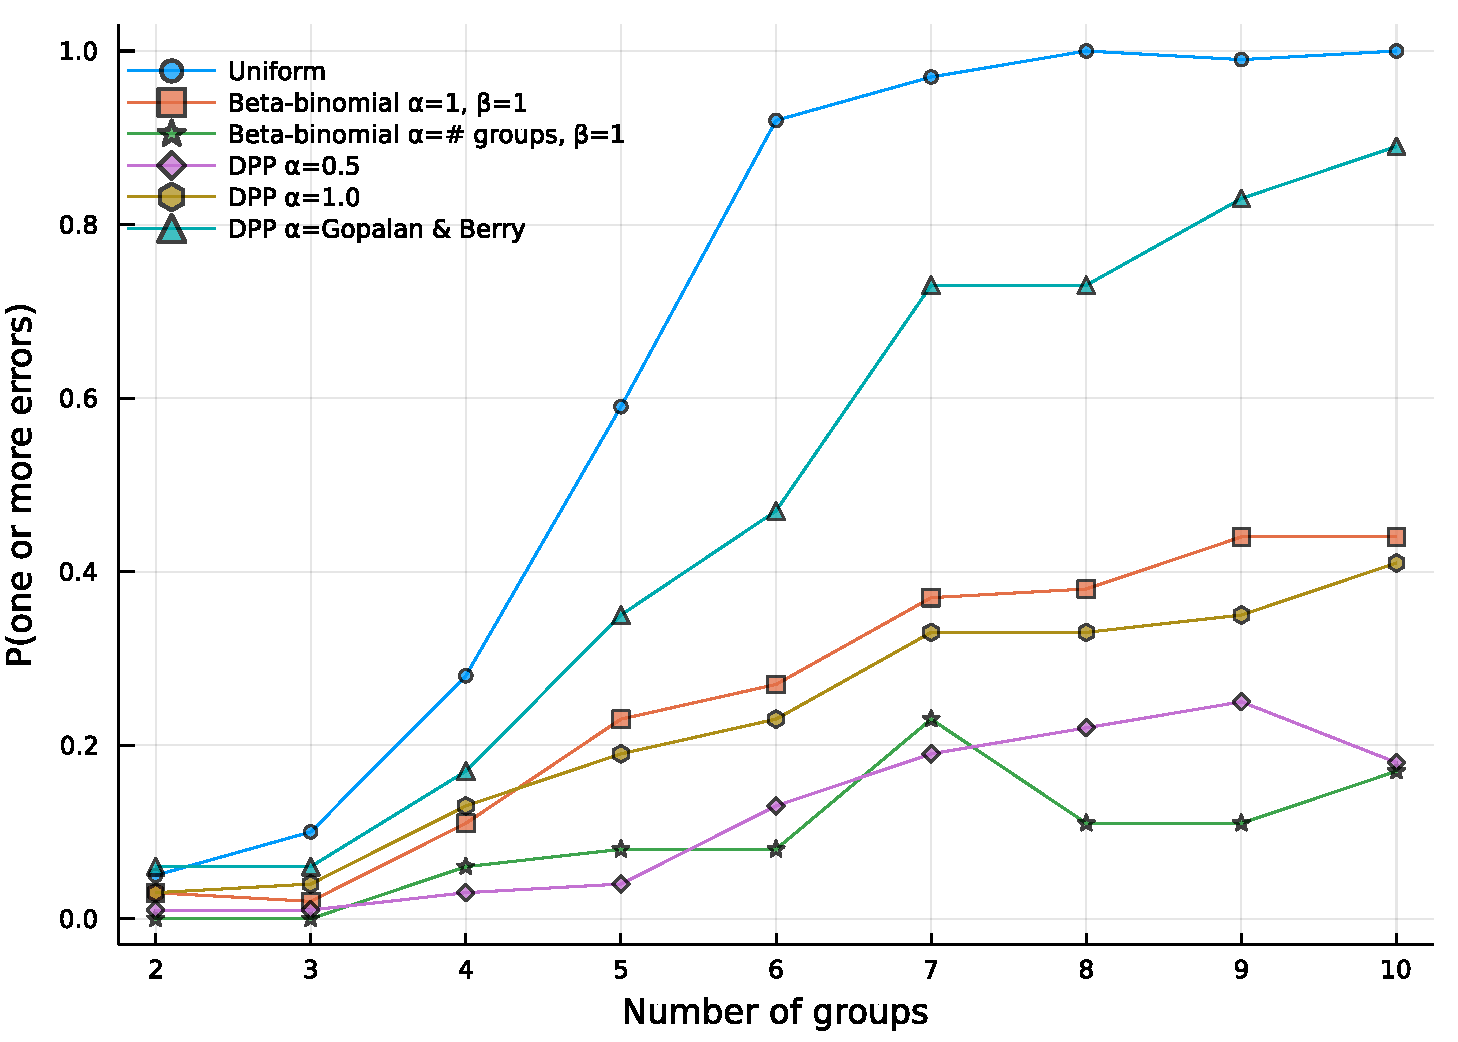
\includegraphics[width=0.90\textwidth]{figures/one_or_more_errors2.pdf}
    \caption{Probability of making one or more errors (left) and rate of errors (right) as a function of the number of groups $K$ for different priors; see main text for details.}
    \label{fig:small_simulation}
\end{figure}
We find that the uniform prior (blue line) result in a high proportion of errors as the number of groups increases. This is not surprising: the uniform prior assigns each model the same prior mass, hence diminishing the plausibility assigned to $\mathcal{H}_0$ dramatically as $K$ increases, thus increasing the frequency of errors. The DP prior which specifies that $p(\mathcal{H}_0) = p(\mathcal{H}_1)$ performs slightly better, but also does not provide adequate multiple comparison adjustment. The beta-binomial prior with $\alpha = 1$ and $\beta = 1$ performs similar to the DP with $\alpha = 1$, but for both the probability of at least one error reaches about 40\% for $K = 10$. As expected from our discussion of Figure \ref{fig:prior-comparison}, the DP prior with $\alpha < 1$ (purple line) and the beta-binomial prior with $\alpha = K$ and $\beta = 1$ (green line) --- both resulting in a monotonically decreasing prior on the number of inequalities --- provide the best error control.


\subsection{Simulation Study} \label{sec:simulation}
In the previous section, we illustrated the importance of the prior in reducing the error rate when all groups are equal. Here we explore the multiplicity adjustment of different priors in a more exhaustive simulation study. We used the same ANOVA model as in the previous section and varied the total number of groups $K \in \{5, 9\}$ and the sample size per group $n \in \{100, 250, 500, 750, 1000, 10000\}$. In addition, we varied the true number of equalities to be $\{25\%, 50\%, 75\%, 100\%\}$. For $K = 5$, there are 4 possible (in)equalities which resulted in models that have either 1, 2, 3, or 4 equalities. For $K = 9$, there are 8 possible (in)equalities, resulting in 2, 4, 6, or 8 equalities in the true model. Given the number of equalities, we picked a particular partition uniformly from all possible partitions with that amount of equalities and used this model to simulate data from. Each unique combination was repeated 100 times and each generated data set was analyzed with the following default priors: the DP prior with $\alpha = 0.50$; the beta-binomial with $\alpha = K$ and $\beta = 1$; and the uniform prior. 

\begin{figure}
    \centering
    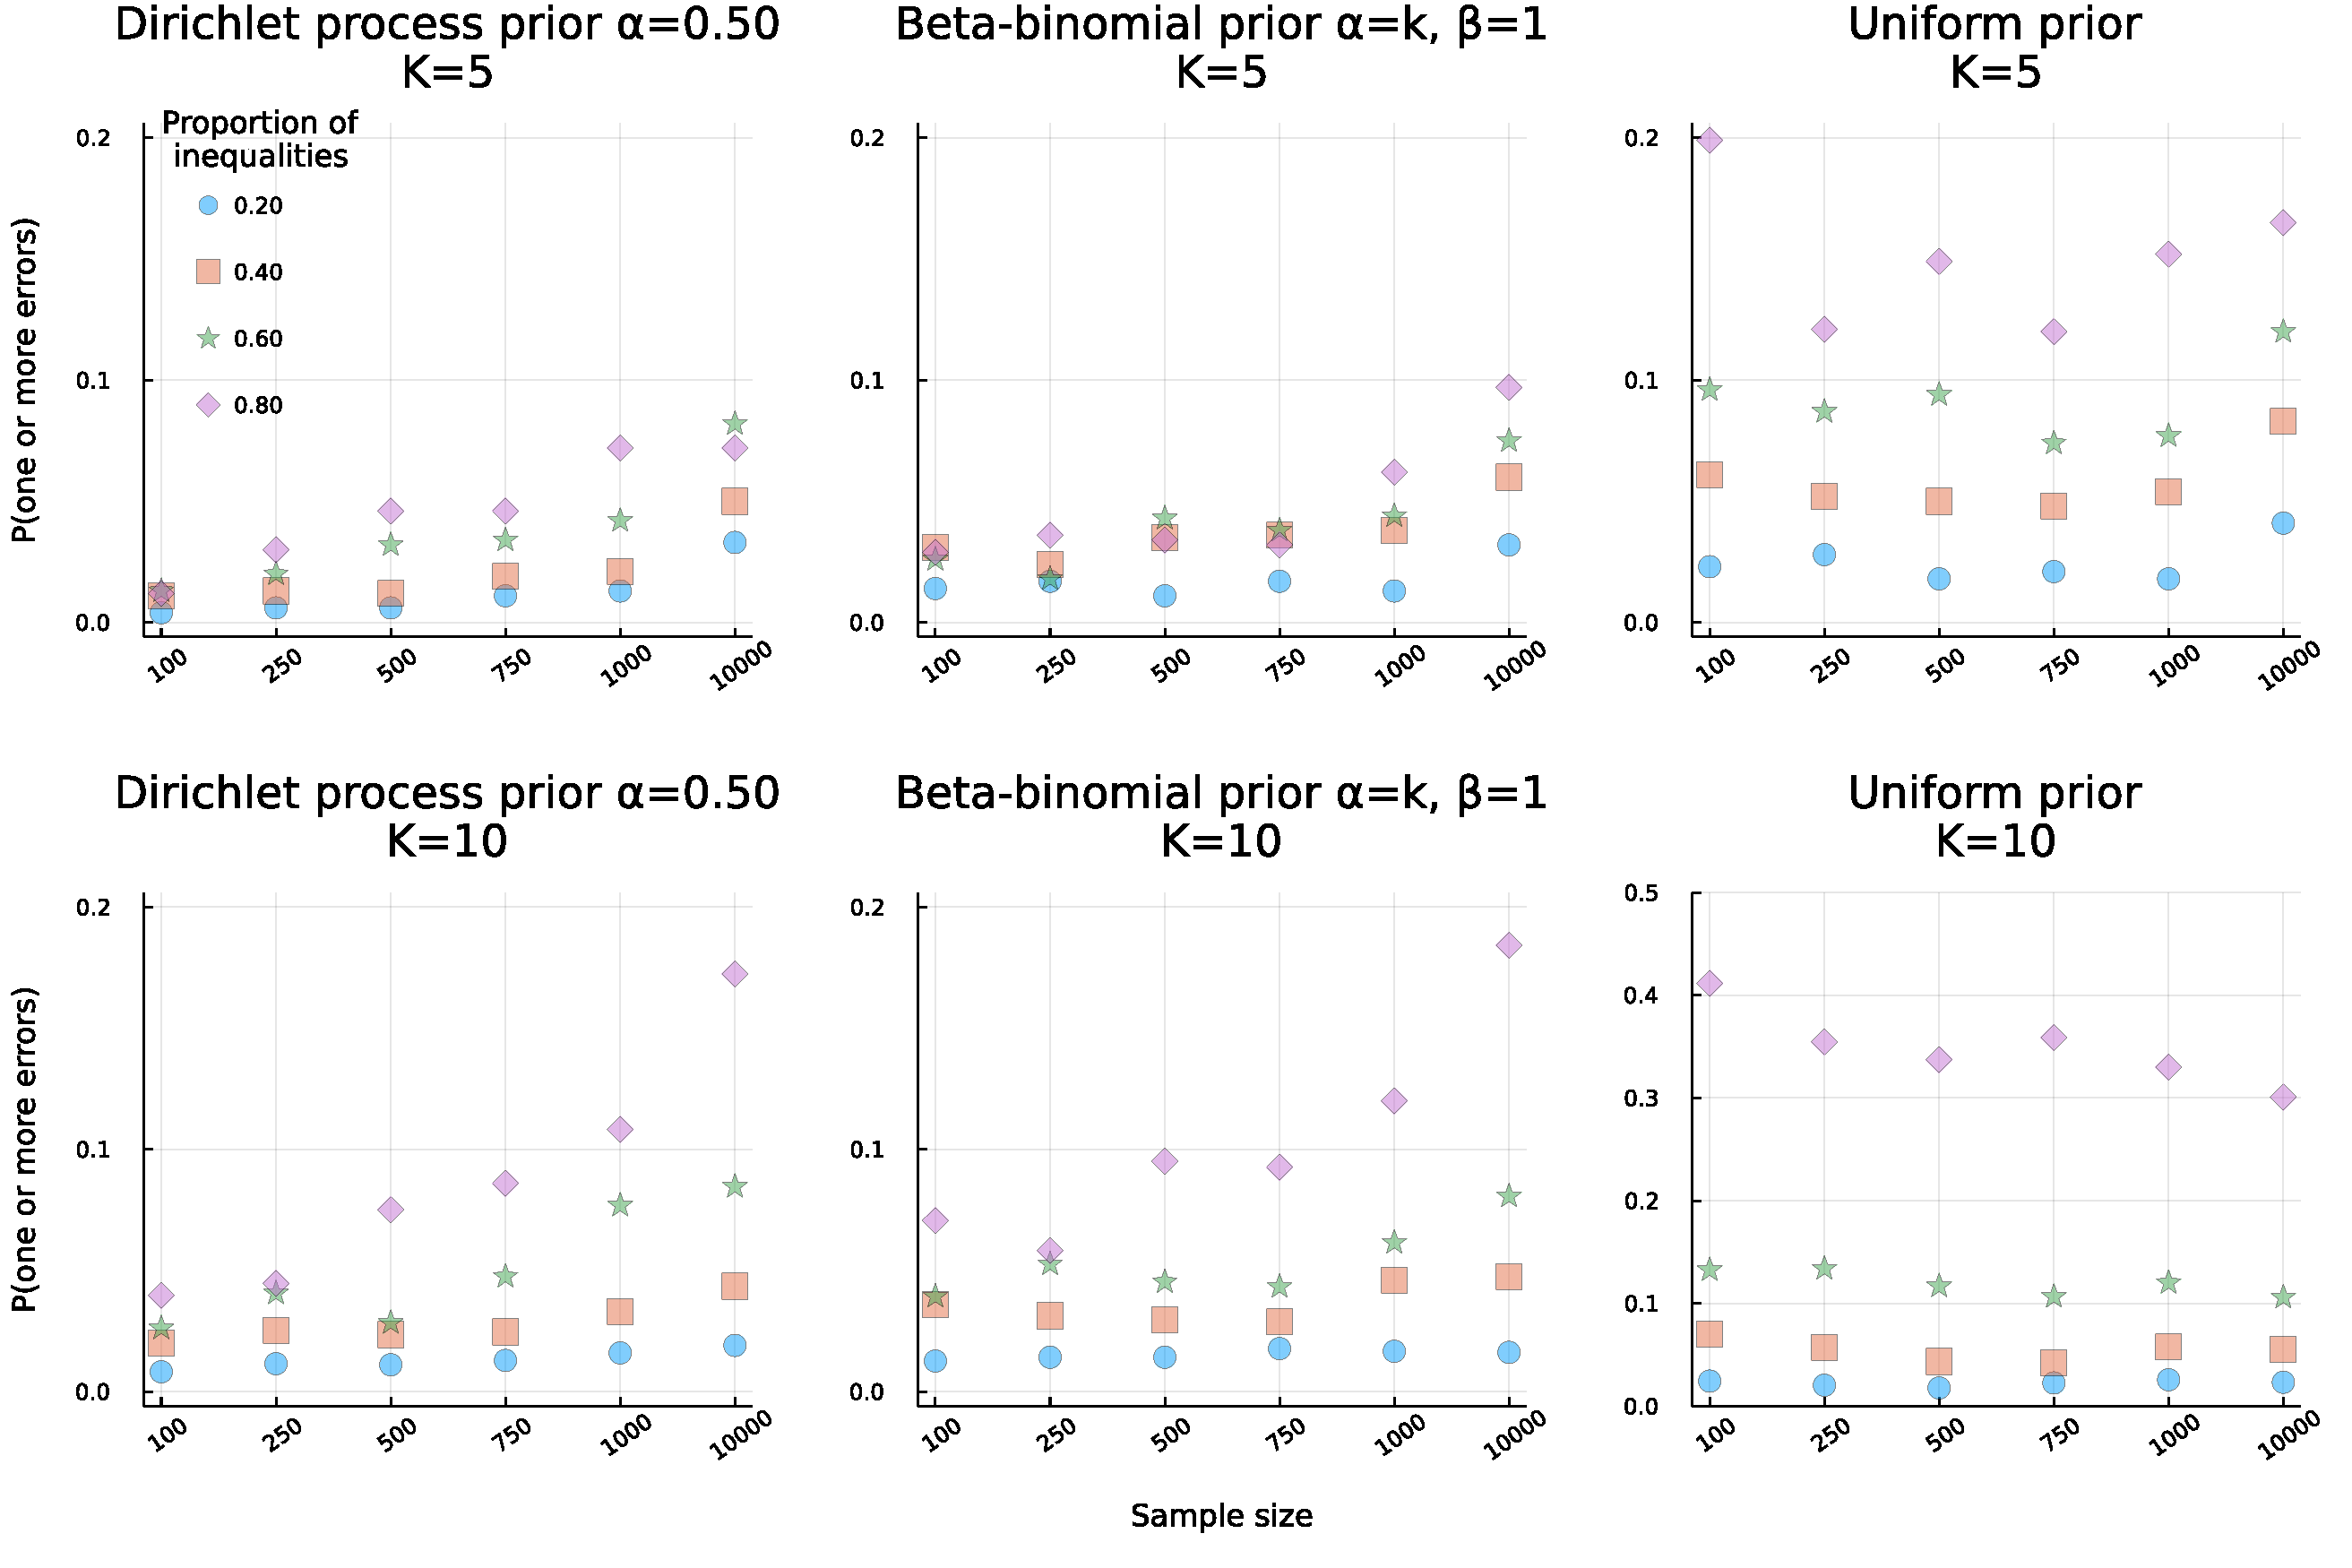
\includegraphics[width=0.95\textwidth]{figures/simulation_results_test_clean_figures/simulation_manuscript.pdf}
    \caption{Proportions of at least one error across priors, sample size, and the proportion of true inequalities. \FD{Nice! I'd still increase font-size of the axis labels and titles, and capitalize the $k$ in the beta-binomial title.}}
    \label{fig:big_simulation}
\end{figure}

Two observations are immediately obvious from Figure \ref{fig:big_simulation}. First, the probability of claiming that two groups are unequal when they are in fact equal increases as the true number of equalities increases (from blue to purple). This holds for all priors, and it makes sense: more equalities implies more opportunities for errors. The second observation is that, while the uniform prior tends to result in more errors, this is most pronounced when the true model has no inequalities; at smaller values, the uniform prior does not perform markedly worse than either the DP prior or the beta-binomial prior.

\section{Applications} \label{sec:applications}
We have created generic Julia and R packages called \textit{EqualitySelection} that utilize the probabilistic programming framework \textit{Turing.jl} to allow the user to adjust for multiplicity. In the following sections, we illustrate the method on two examples: testing the (in)equality of proportions and variances, respectively; the code to reproduce the results is given in Appendix \ref{sec:appendix-code}.


\iffalse
\subsection{Testing Means}
Intrusive memories after a traumatic experience can noticeably affect somebody's mental health. \textcite{james2015computer} tested whether intrusive memories can be reduced by simple cognitive task after memory consolidation. In particular, they had people watch a scary movie and after seven days report the number of intrusive memories they had. There were four experimental conditions applied one day after the scary movie, to allow for the memory to be consolidated. In the ``no-task'' control group, participants completed a filler task after watching the scary movie; in the ``Tetris only'' group, participants played Tetris; in the ``Reactivation only'' group, participants were presented with images from the scary movie; and, lastly, the ``Reactivation + Tetris'' condition had participants play Tetris after the reactivation task.

% http://environmentalcomputing.net/analysis-variance-single-factor/
% https://crumplab.github.io/statistics/anova.html

%\textcite{gopalan1998bayesian} analyze a nice $k = 6$ ANOVA data set but with only $n = 5$ per group.

\FD{Problem is that it's count data ... hmmm.}
\FD{Since we already have a Demo using the ANOVA model, we could leave this out.}
\fi

%\textcite{tong2008too} have five groups rate attractiveness of Facebook users with 100, 300, 500, 700, 900 friends, respectively. Nice example, but a bit dated; it's in JASP.

\subsection{Testing Proportions}
\textcite{nuijten2016prevalence} investigated a sample of 30,717 articles published between 1985 and 2013 in eight major psychology journals for statistical reporting errors. Our question here is: Which journals make the same amount of errors, and which make more errors? We implement the model as follows. For journal $j$, denote the number of statistical errors found as $e_j$ and the number of statistical tests analyzed as $n_j$. We assume that underlying each proportion there is a latent true chance of making an error, $\theta_j$. Thus, the data are modeled as independent binomials, that is, $e_j \sim \mathrm{Binomial}\left(\theta_j, n_j\right)$. Next, we specify a hierarchical level over the partitions to assess for which journals the chances of making an error are equal. This leads to the following model specification:
\begin{align*}
    e_j                 &\sim \mathrm{Binomial}\left(\theta_j, n_j\right)\\
    \theta^u_j          &\sim \text{Beta}(1, 1)\\
    \theta_j            &\leftarrow \theta^u_i \quad\text{ iff } j \in \rho_i\\
    \rho                &\sim \pi(.) \enspace . \numberthis
\end{align*}
The unconstrained chances $\theta^u_j$ are assigned a Beta prior, from which, together with the partitions, the possibly constrained chances are created. Two chances, $\theta_i$ and $\theta_j$, are equal if and only if their indices appear in the same partition, $\{i, j\} \subseteq \rho_k$ for some $k$. Note that the model reduces to the full model of independent binomials whenever the partitions state that all $\theta$s are distinct. Figure~\ref{fig:demo_proportions} shows the effect of allowing different error chances to be equal. The left panel shows the results for the full model --- the observer proportions and posterior means are in near perfect agreement. The right panel shows the results for a default beta-binomial prior with $\alpha = 8$, $\beta = 1$ prior, illustrating that adjusting for multiplicity introduces shrinkage in the parameter estimates towards each other. 
\begin{figure}
    \centering
    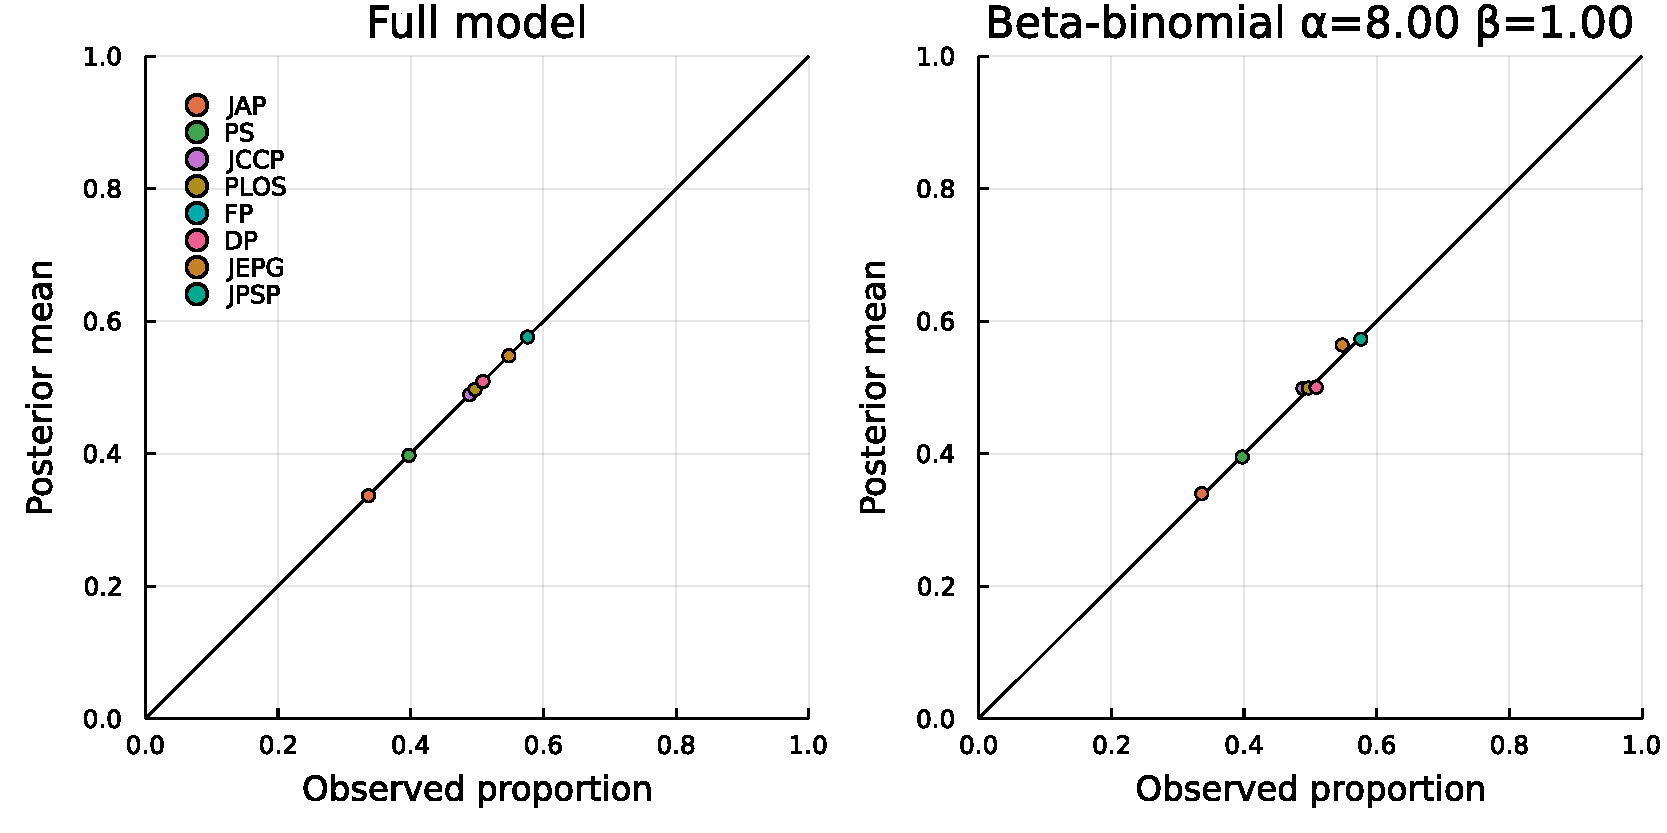
\includegraphics[width=\textwidth]{figures/demo_proportions_retrieval_plots_full_bb.pdf}
    \caption{Left: Posterior means of the full model where all proportions are assumed the be different. Right: Posterior means with a beta-binomial prior over the partitions with $\alpha = 8$ and $\beta = 1$. The abbreviations stand for: 
    \emph{Journal of Applied Psychology} (JAP), \emph{Psychological Science} (PS), \emph{Journal of Consulting and Clinical Psychology} (JCCP), \emph{ Public Library of Science} (PLOS), \emph{Developmental Psychology} (DP), \emph{Journal of Experimental Psychology: General} (JEPG), and \emph{Journal of Personality and Social Psychology} (JPSP).}
    \label{fig:demo_proportions}
\end{figure}

%\FD{How is the model implemented? Is it like ANOVA, but on proportions? Then it would be log linear analysis. \textcite{gopalan1998bayesian} just compare proportions, for example. It seems that the Bayesian loglinear analysis in JASP (due to Overstall \& Forster) does model averaging, so in a sense it should be very similar to our approach. It also makes more sense conceptually, see the example below.}
%\textcite{radelet1991choosing} study decisions on death penalties (yes / no) by race of defendant (black / white) and race of victim (black / white). This yields 6 cells, data are in JASP. An interaction in a loglinear model would have a particular effect on the posterior equivalence of groups, so there is some relation here. Let's discuss this.

%There is another nice data set about bias in MOOCs due to \textcite{baker2018bias}, but the JASP data set completely ignores variance due to different MOOCs, instructors, etc. So it's a completely inadequate analysis.


\subsection{Testing Variances}
\textcite{dablander2020default} developed a default Bayes factor test for testing the (in)equality of variances. Here, we extent their model specification with our beta-binomial model prior, which results in:
\begin{align*}
    Y_{ij}                   &\sim \mathcal{N}\left(\mu_j, \left(2\vartheta_j\tau\right)^{-1}\right)\\
    \mu_j                    &\propto 1  \\
    \tau                     &\propto \tau^{-1} \\
    \vec{\vartheta}^u     &\sim \text{Dirichlet}(1, \ldots, 1) \\
    \vartheta_j              &\leftarrow \vartheta^u_i \quad\text{ iff } j \in \rho_i \\
    \rho                     &\sim \pi(.) \enspace , \numberthis
\end{align*}
where $\tau$ is the grand precision and $\vartheta$ is the $K$-dimensional vector of mixture weights such that $\sigma_j^2 = \tau_j^{-1} = \left(2\vartheta_j\tau\right)^{-1}$; for details, see \textcite{dablander2020default}.

%\textcite{boos2004comparing} reanalyze a data set with 8 groups concerning pheromones and flowers reported in \textcite{groot2005effect}; pretty boring, but something like this we need. Hmm, but they only report absolute deviation from the mean, not the sample variances. See \url{https://www.tandfonline.com/doi/abs/10.1080/03610918.2018.1485937?journalCode=lssp20} for variance test from 1994 on four groups.
% https://onlinelibrary.wiley.com/doi/full/10.1002/ldr.2816

\section{Discussion} \label{sec:discussion}
Testing the (in)equality among groups while adjusting for multiple comparisons is a core challenge in many applied settings. In this paper, we have proposed a flexible class of beta-binomial priors to penalize multiplicity and make inferences over all possible (in)equalities in relatively general settings. We compared our prior to a Dirichlet process prior suggested by \textcite{gopalan1998bayesian} and to a uniform prior. We showed in simulations that a beta-binomial prior with $\alpha = K$ and $\beta = 1$ as well as a Dirichlet process prior with $\alpha < \nicefrac{1}{2}$ controls the probability of incorrectly claiming that true groups are unequal, while a uniform prior, as expected, generally does not. Lastly, we also illustrated our method, which is freely available in the Julia and R packages \textit{EqualitySelection}, on three examples. In contrast to conventional adjustments for multiple comparisons \parencite[e.g.,][]{westfall1997bayesian, jeffreys1961theory}, our method makes inferences over all possible (in)equalities. This means that researchers can use it to assess not only the probability of pairwise (in)equalities --- as is common in standard post-hoc tests for, say, ANOVA --- but in fact can make probabilistic statements over any set of (in)equalities they wish assess.

As with any new method, there are a number of points to keep in mind. First, our method is fairly flexible, and while we suggest default values of $\alpha = K$ and $\beta = 1$ for the beta-binomial prior and $\alpha = \nicefrac{1}{2}$ for the DP prior, researchers may wish to use more informed ones. In some sense, the DP prior is more constrained, requiring, as we have shown, that $\alpha < 1$ in order to penalize multiplicity. Second, the beta-binomial prior differs from the DP prior in that it assigns models with the same number of partitions the same prior probability, while the DP prior assigns more mass to the model with the larger partition. It is not obvious which of the two behaviours is more desirable, and may well depend on the problem under study. Researchers using the methods we have made available should keep this difference in mind, although it is unlikely to matter much in practice. Third, only reducing the probability of incorrectly claiming that two groups are different when in fact they are not is not necessarily the best strategy. Instead, it is important to also study the extent to which the method does not pick up differences that are in fact there. \FD{We should do this simulation study, let's discuss.}

There are also a few practical limitations of our proposed method that we leave for future work. We currently do not allow for factorial designs, for which a dummy coding is more natural, and we do not allow for dependent observations. Extending the method to allow for dependent observations is fairly straightforward, requiring only a change in the likelihood. Incorporating factorial designs is more tricky, however.

%\textcite{kim2009spiked} combine a spike at zero with a DPP. \textcite{curtis2011bayesian} also use a DPP to combine clustering of highly correlated predictors in linear regression with variable selection. \textcite{canale2017pitman} focus on the Pitman-Yor process, which is a generalization of the DPP. \textcite{lu2018reducing} study a powered Chinese restaurant process. \textcite{miller2015microclustering} study a microclustering property, for which the number of data points in a cluster does not grow linearly with the total number of data points (which is assumed by the DP, PY, etc.)

% We focused on independent groups, but one could model dependencies using the distance CRP \parencite{blei2011distance}.

%The Pitman-Yor process generalizes the DP \parencite{pitman1997two}, but it, too, assumes a ``rich-get-richer'' structure which may be undesirable. Both the DP and the PY are instances of so-called \textit{species-sampling models} (SSM), which are a general class of nonparametric models \parencite[e.g.,][]{lee2013defining, ishwaran2003generalized, pitman1996some}. To keep this paper contained, however, we focus on the DP as the only example of a nonparametric model.

\iffalse
Discussion points:
\begin{itemize}
    \item Factorial designs
    \begin{itemize}
        \item Here a dummy coding is more natural, which does not square with our setup. Maybe fine if we combine offsets?
    \end{itemize}
    \item Dependent observations
    \begin{itemize}
        \item Either a relatively simple (?) change to the likelihood, or a time-series problem
    \end{itemize}
    \item DP and BB partition difference
\end{itemize}
\fi

\iffalse
\subsection{Convergence Rate}
\begin{itemize}
    \item \textcolor{red}{For each prior, simulate from true model and plot posterior probability as sample size increases. Ideally, we see that DP is not consistent.}
\end{itemize}

\FD{We should do this plot just to check the consistency result from above, but I'm not sure whether it should actually be in the paper. I mean, it will just show the (slow) Bayes factor convergence.}

\textcite{chen1995optimal} showed that the optimal rate of convergence in the finite mixture problem when the number of components are unknown is $n^{-\frac{1}{4}}$ (with knowledge of the components, the rate can be $\sqrt{n}$). \textcite{ishwaran2001bayesian} show that a Bayesian estimation method is consistent and achieves the $n^{-\frac{1}{4}}$ convergence rate in finite mixtures with the number of components unknown.

\textcite{miller2014inconsistency} argue that nonparametric clustering using a large class of models is inconsistent; see also \textcite{miller2013simple}, for an example. \textcite{miller2018mixture} therefore suggest mixture models with a prior on the number of components with support $\mathbb{N}$ instead of using a nonparametric approach. See also \textcite{green2001modelling} for a comparison of the two approaches.
\fi


\printbibliography

\newpage
\appendix

\section{Example Code} \label{sec:appendix-code}
Using the Julia language, the code below reproduces the results in Section \ref{sec:applications}.

\begin{minted}{Julia}
using Package; Pkg.add("EqualitySelection.jl")
using EqualitySelection
\end{minted}

\noindent This can also be done from R, as the code below demonstrates.

\begin{minted}{R}
devtools::install_github('vandenman/EqualitySelection')
library('EqualitySelection')
\end{minted}

\iffalse
\newpage
\begin{figure}
    \centering
    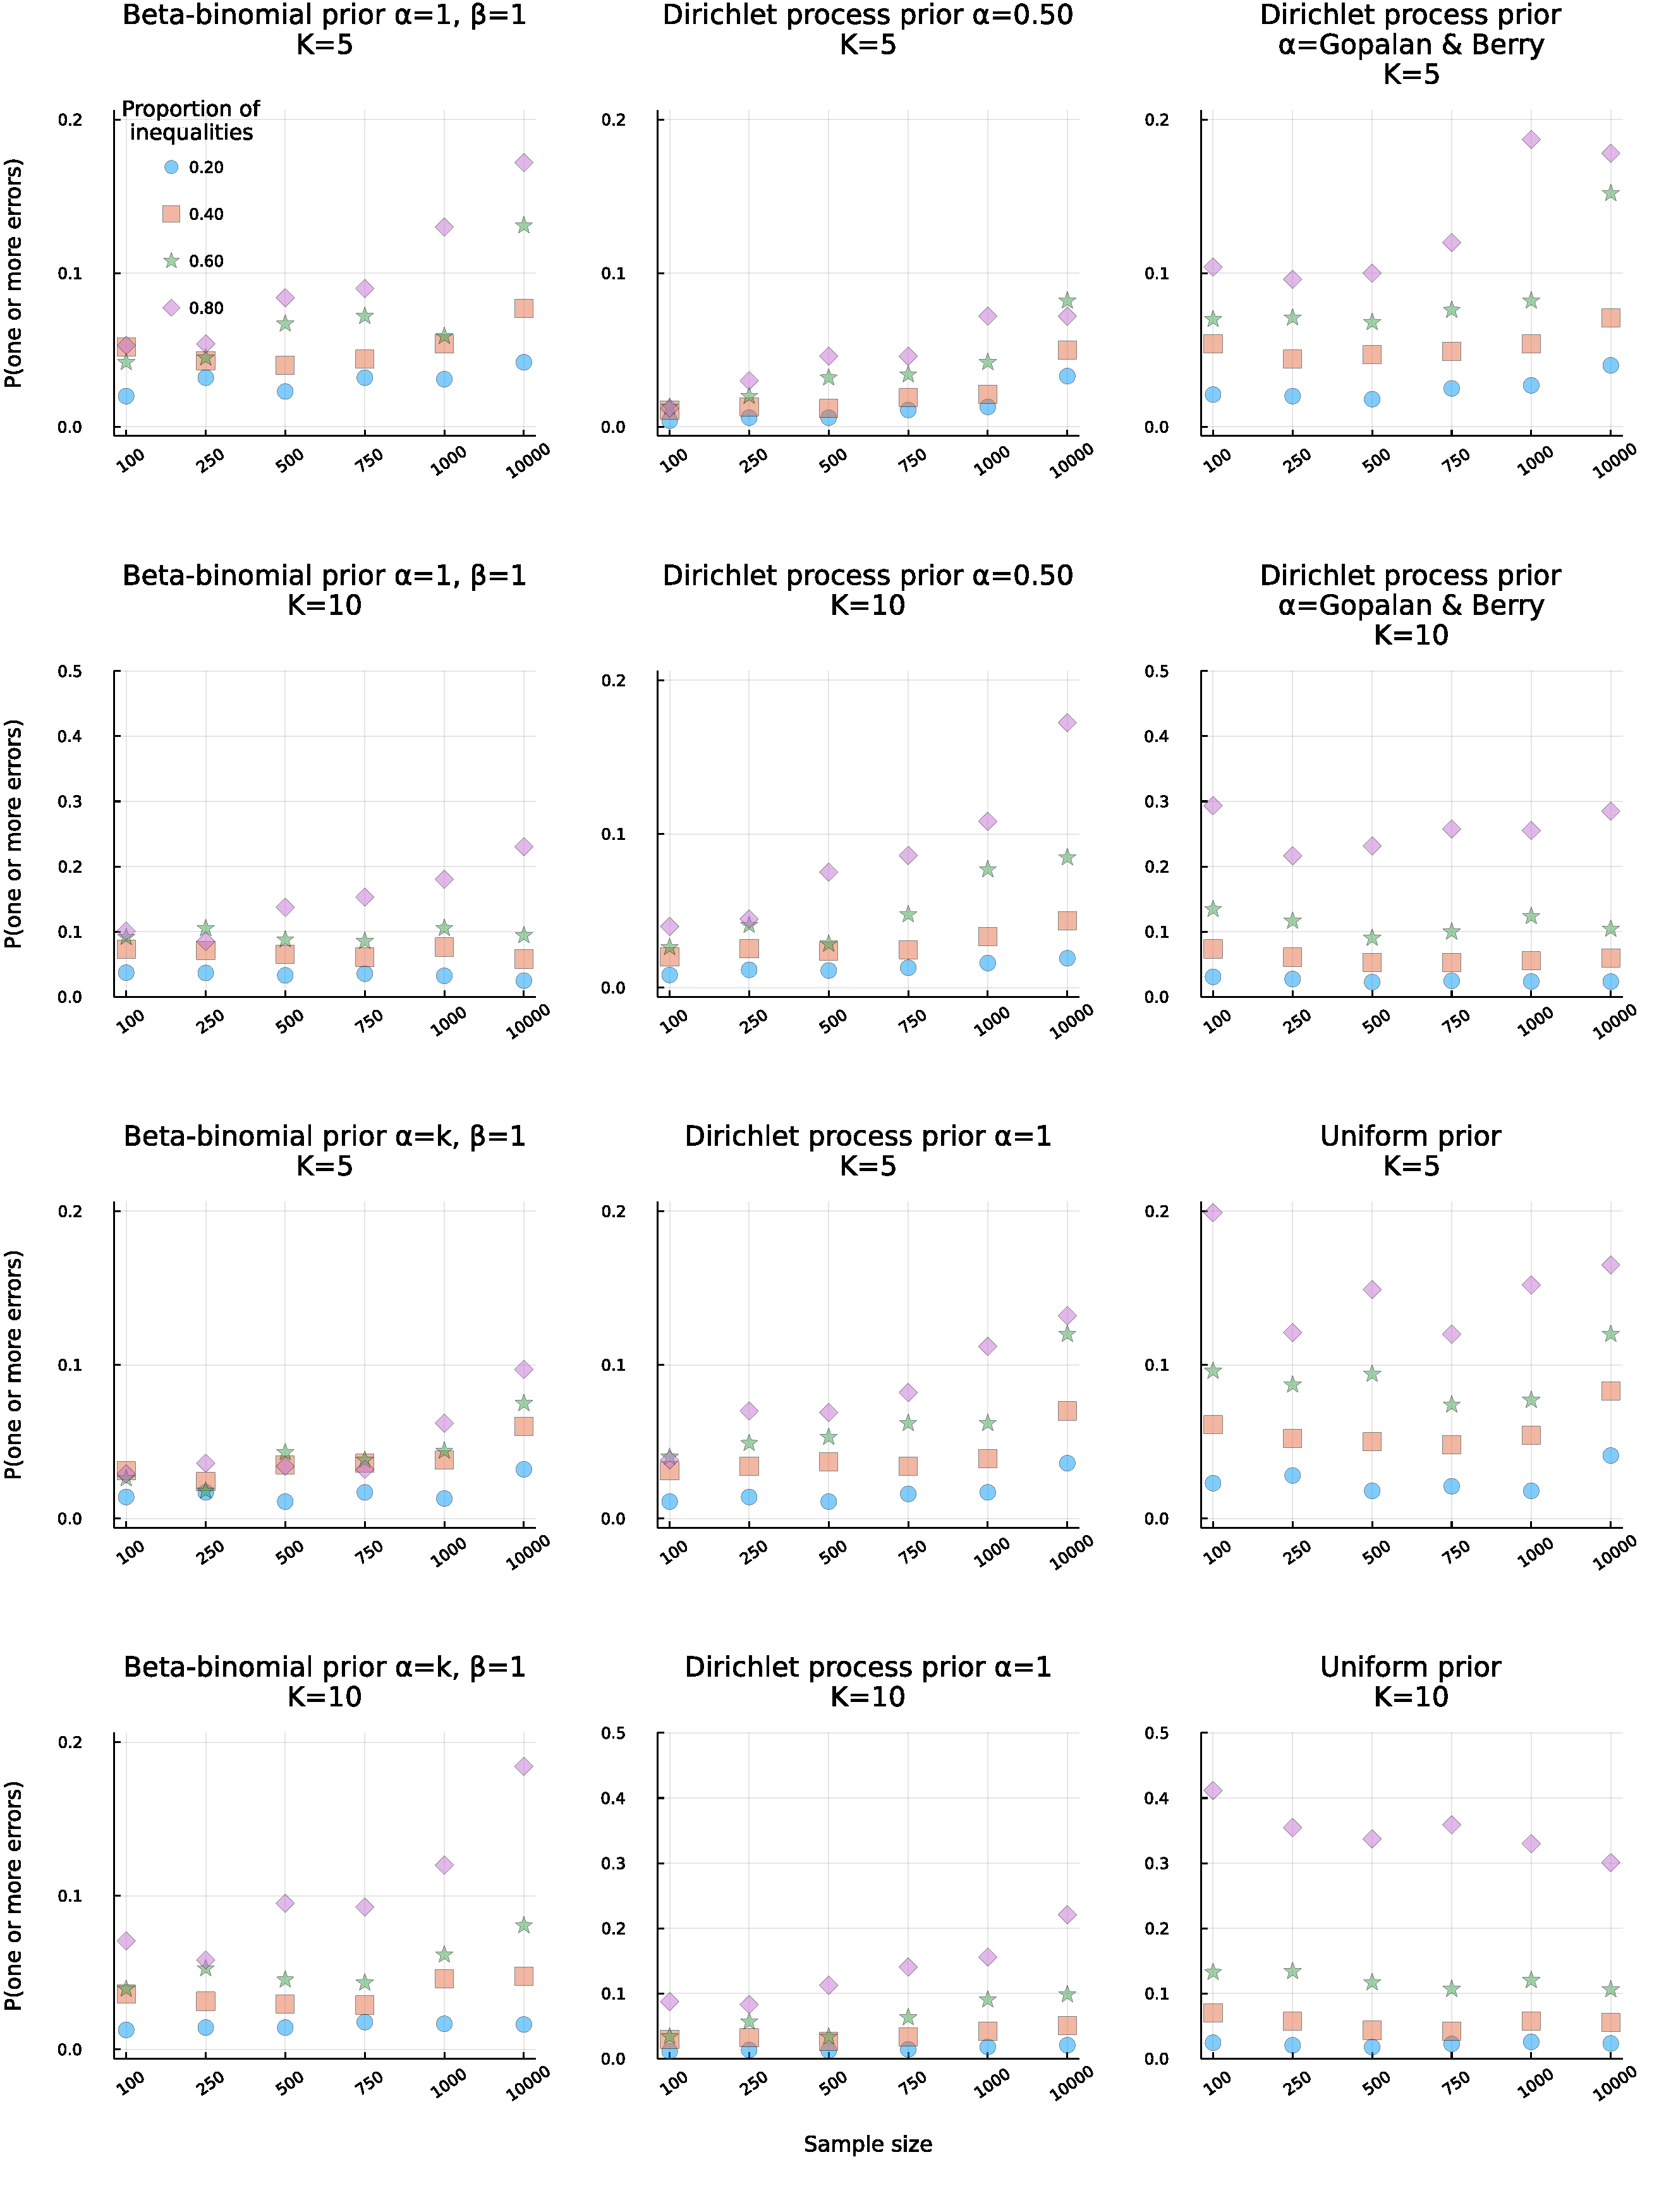
\includegraphics[width=\textwidth]{figures/simulation_results_test_clean_figures/simulation_appendix.pdf}
    \caption{Proportion of false inequalities recovered across all simulations.}
    \label{app_fig:big_simulation}
\end{figure}
\fi

\end{document}
